\documentclass[letterpaper, 12pt]{article}

\usepackage{amsmath, amsthm, amssymb, dsfont, accents}
\usepackage{hyperref, subcaption, booktabs}
\usepackage{fullpage}

\usepackage{tikz, pgfplots}
\pgfplotsset{compat=newest}
\newlength{\figurewidth}
\newlength{\figureheight}

\newcommand{\argmin}{\operatornamewithlimits{arg\ min}}
\newcommand{\argmax}{\operatornamewithlimits{arg\ max}}
\newcommand{\ind}[1]{\mathds{1}_{{#1}}} 
\newcommand{\ubar}[1]{\underaccent{\bar}{#1}}

\title{Invariant Set Lane Keeping Controller Explained}
\author{Petter Nilsson \\ \href{mailto:pettni@umich.edu}{pettni@umich.edu}}

\begin{document}

\section{Model} % (fold)
\label{sec:model}

The controller is designed for the following 3-state model:

\begin{equation}
	\begin{bmatrix}
		\dot y \\
		\dot \psi \\
		\dot r
	\end{bmatrix}
	= 
	\begin{bmatrix}
		0 & u_0 & 0 \\
		0 & 0   & 1 \\
		0 & 0 & - \frac{a^2 C_{\alpha f} + b^2 C_{\alpha r}}{I_z u_0}
	\end{bmatrix} 
	\begin{bmatrix}
		y \\
		\psi \\
		r
	\end{bmatrix}
	+ 
	\begin{bmatrix}
		0 \\ 0 \\ \frac{a C_{\alpha f}}{I_z}
	\end{bmatrix}
	\delta_f
	+ \begin{bmatrix}
		0 & 1 \\
		1 & 0 \\
		0 & \frac{b C_{\alpha r} - a C_{\alpha f}}{I_z u_0}
	\end{bmatrix} 
	\begin{bmatrix}
		r_{road} \\
		v
	\end{bmatrix}
\end{equation}

and implemented on the 4-state model

\begin{equation}
	\begin{bmatrix}
		\dot y \\
		\dot r \\
		\dot \psi \\
		\dot r
	\end{bmatrix}
	= 
	\begin{bmatrix}
	0 & 1 & u_0 & 0 \\
    0 & -\frac{C_{\alpha f}+C_{\alpha r}}{m u_0}  & 0 & \frac{b C_{\alpha r}-a C_{\alpha f}}{m u_0} - u_0 \\
    0 & 0 & 0 & 1 \\
    0 & \frac{b C_{\alpha r}-a C_{\alpha f}}{I_z u_0} & 0 & - \frac{a^2   C_{\alpha f} + b^2   C_{\alpha r}}{Iz u_0}
	\end{bmatrix} 
	\begin{bmatrix}
		y \\
		v \\
		\psi \\
		r
	\end{bmatrix}
	+ 
	\begin{bmatrix}
		0 \\ \frac{C_{\alpha f}}{m} \\ 0 \\ \frac{a C_{\alpha f}}{I_z}
	\end{bmatrix}
	\delta_f
	+ \begin{bmatrix}
		0 \\
		0 \\
		1 \\
		0 
	\end{bmatrix} 
		r_{road} 
\end{equation}

% section model (end)

\section{Disturbance assumptions} % (fold)
\label{sec:assumptions}

Maximal road curvature: 
\begin{equation}
	r_{road} \in [- \alpha \frac{g}{u_0}, \alpha \frac{g}{u_0}]
\end{equation}

Modeling error due to setting $v=0$:
\begin{equation}
	v \in [-1, 1]
\end{equation}

% section assumptions (end)

\section{Specifications} % (fold)
\label{sec:specifications}

Don't exit the lane:
\begin{equation}
	\square (y \in [-0.9, 0.9])
\end{equation}

% section specifications (end)

\setlength\figurewidth{0.4\columnwidth} 
\setlength\figureheight{0.3 \columnwidth} 

\begin{figure}[h]
	\begin{center}
		% 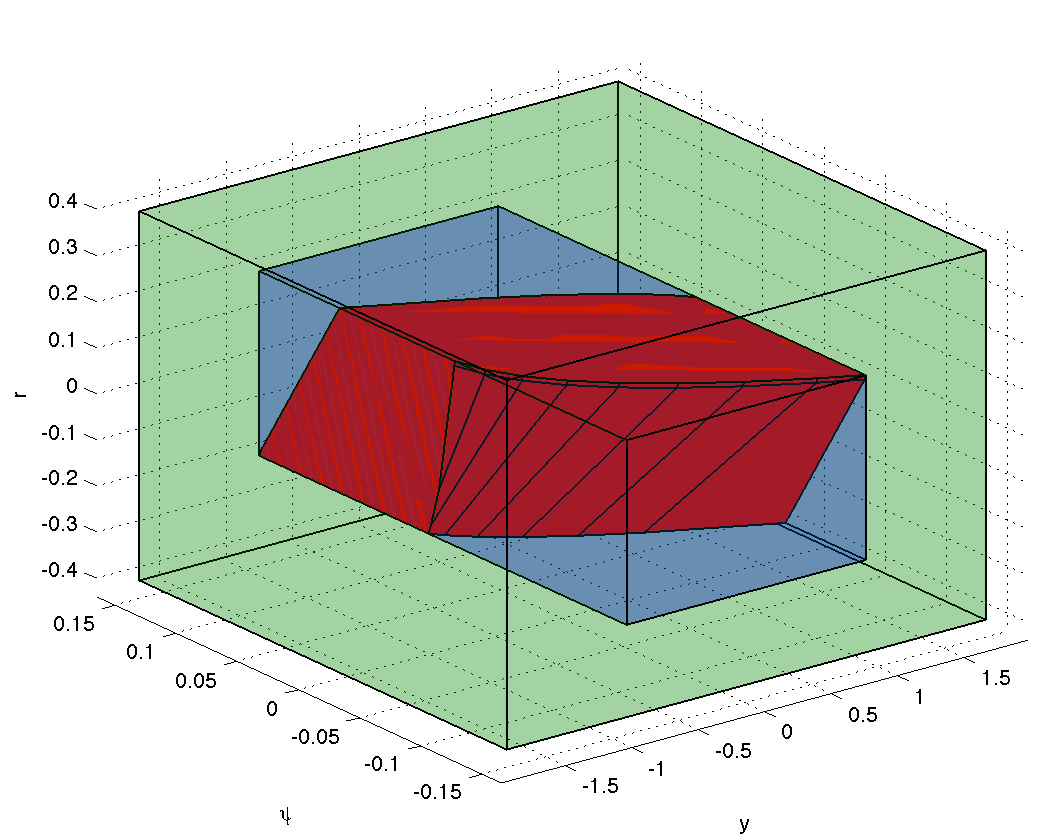
\includegraphics[width=0.4\columnwidth]{invariant}
		% This file was created by matlab2tikz v0.4.7 running on MATLAB 8.2.
% Copyright (c) 2008--2014, Nico Schlömer <nico.schloemer@gmail.com>
% All rights reserved.
% Minimal pgfplots version: 1.3
% 
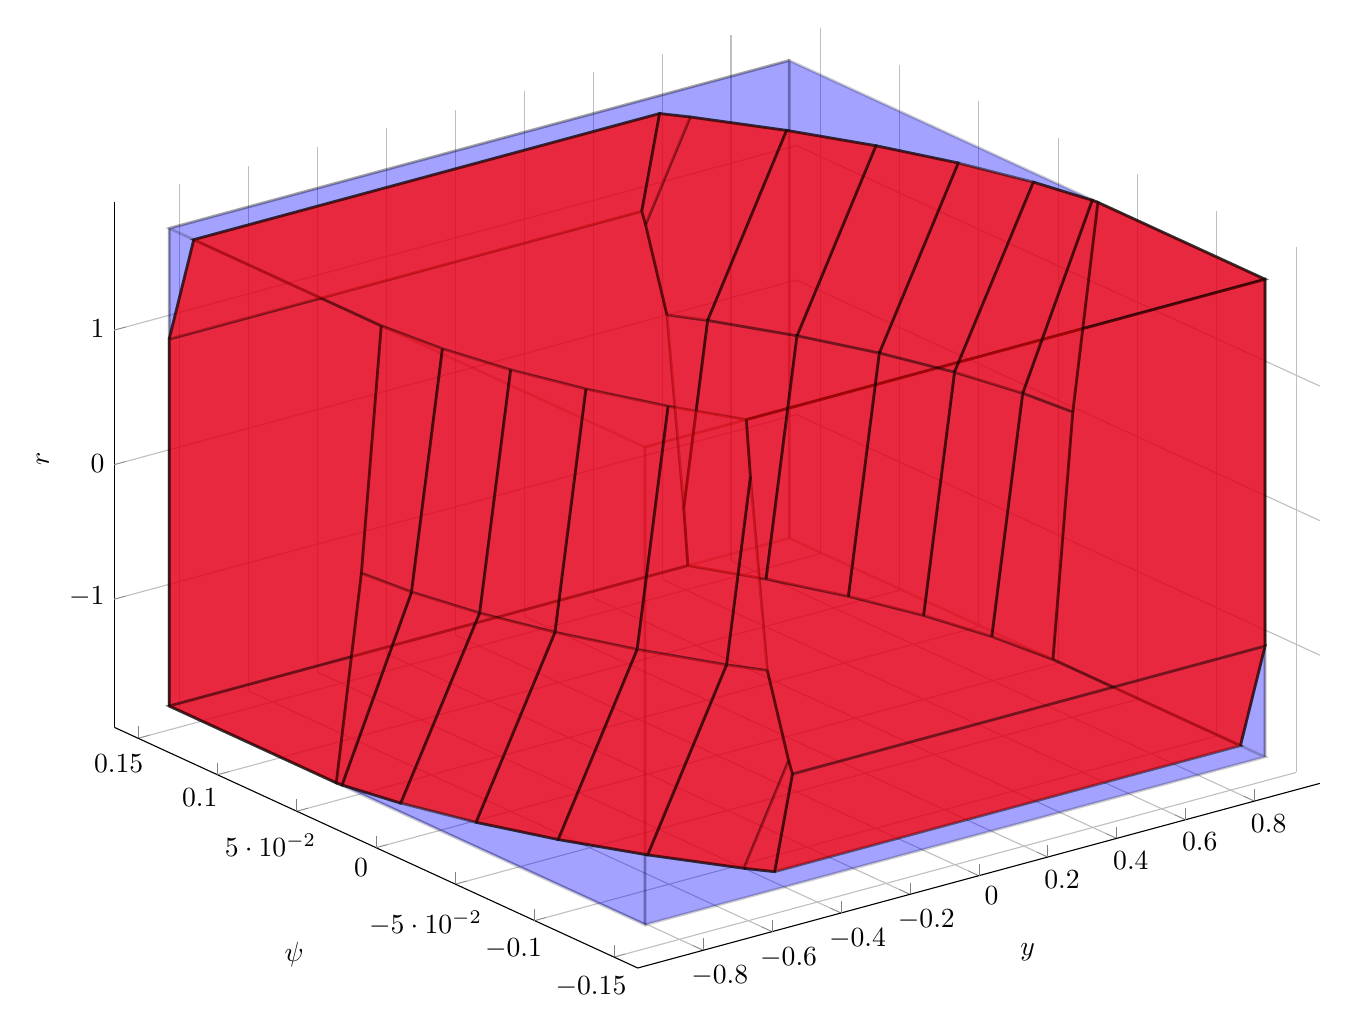
\begin{tikzpicture}

\begin{axis}[%
width=6.02777777777778in,
height=4.75416666666667in,
view={-37.5}{30},
scale only axis,
xmin=-0.99,
xmax=0.99,
xlabel={$y$},
xmajorgrids,
ymin=-0.165,
ymax=0.165,
ylabel={$\psi$},
ymajorgrids,
zmin=-1.95299910967934,
zmax=1.95299910967934,
zlabel={$r$},
zmajorgrids,
axis x line*=bottom,
axis y line*=left,
axis z line*=left
]

\addplot3[area legend,solid,line width=1.0pt,fill=blue,opacity=2.000000e-01,draw=black,forget plot]
table[row sep=crcr] {%
x	y	z\\
0.9	-0.15	-1.77545373607212\\
0.9	-0.15	1.77545373607212\\
0.9	0.15	1.77545373607212\\
0.9	0.15	-1.77545373607212\\
};


\addplot3[area legend,solid,line width=1.0pt,fill=blue,opacity=2.000000e-01,draw=black,forget plot]
table[row sep=crcr] {%
x	y	z\\
-0.9	-0.15	1.77545373607212\\
-0.9	-0.15	-1.77545373607212\\
-0.9	0.15	-1.77545373607212\\
-0.9	0.15	1.77545373607212\\
};


\addplot3[area legend,solid,line width=1.0pt,fill=blue,opacity=2.000000e-01,draw=black,forget plot]
table[row sep=crcr] {%
x	y	z\\
0.9	0.15	-1.77545373607212\\
0.9	0.15	1.77545373607212\\
-0.9	0.15	1.77545373607212\\
-0.9	0.15	-1.77545373607212\\
};


\addplot3[area legend,solid,line width=1.0pt,fill=blue,opacity=2.000000e-01,draw=black,forget plot]
table[row sep=crcr] {%
x	y	z\\
0.9	-0.15	1.77545373607212\\
-0.9	-0.15	1.77545373607212\\
-0.9	0.15	1.77545373607212\\
0.9	0.15	1.77545373607212\\
};


\addplot3[area legend,solid,line width=1.0pt,fill=blue,opacity=2.000000e-01,draw=black,forget plot]
table[row sep=crcr] {%
x	y	z\\
-0.9	-0.15	-1.77545373607212\\
-0.9	-0.15	1.77545373607212\\
0.9	-0.15	1.77545373607212\\
0.9	-0.15	-1.77545373607212\\
};


\addplot3[area legend,solid,line width=1.0pt,fill=blue,opacity=2.000000e-01,draw=black,forget plot]
table[row sep=crcr] {%
x	y	z\\
-0.9	-0.15	-1.77545373607212\\
0.9	-0.15	-1.77545373607212\\
0.9	0.15	-1.77545373607212\\
-0.9	0.15	-1.77545373607212\\
};


\addplot3[area legend,solid,line width=1.0pt,fill=red,opacity=5.000000e-01,draw=black,forget plot]
table[row sep=crcr] {%
x	y	z\\
0.9	-0.134460224004354	-1.77545373607212\\
0.9	-0.15	-0.951257668418722\\
0.9	-0.15	1.77545373607212\\
0.9	-0.0445797996829758	1.77545373607212\\
0.9	-0.0287735096778711	0.131430219551011\\
0.9	-0.0162509912512161	-1.77545373607212\\
0.9	-0.0162509912512161	-1.77545373607212\\
0.9	-0.0162509912512161	-1.77545373607212\\
0.9	-0.0162509912512161	-1.77545373607212\\
0.9	-0.0162509912512161	-1.77545373607212\\
0.9	-0.0162509912512161	-1.77545373607212\\
0.9	-0.0162509912512161	-1.77545373607212\\
0.9	-0.0162509912512161	-1.77545373607212\\
0.9	-0.0162509912512161	-1.77545373607212\\
0.9	-0.0162509912512161	-1.77545373607212\\
0.9	-0.0162509912512161	-1.77545373607212\\
};


\addplot3[area legend,solid,line width=1.0pt,fill=red,opacity=5.000000e-01,draw=black,forget plot]
table[row sep=crcr] {%
x	y	z\\
-0.9	0.0162509912512162	1.77545373607212\\
-0.9	0.0287735096778705	-0.131430219550917\\
-0.9	0.0445797996829763	-1.77545373607212\\
-0.9	0.15	-1.77545373607212\\
-0.9	0.15	0.951257668418724\\
-0.9	0.134460224004354	1.77545373607212\\
-0.9	0.134460224004354	1.77545373607212\\
-0.9	0.134460224004354	1.77545373607212\\
-0.9	0.134460224004354	1.77545373607212\\
-0.9	0.134460224004354	1.77545373607212\\
-0.9	0.134460224004354	1.77545373607212\\
-0.9	0.134460224004354	1.77545373607212\\
-0.9	0.134460224004354	1.77545373607212\\
-0.9	0.134460224004354	1.77545373607212\\
-0.9	0.134460224004354	1.77545373607212\\
-0.9	0.134460224004354	1.77545373607212\\
};


\addplot3[area legend,solid,line width=1.0pt,fill=red,opacity=5.000000e-01,draw=black,forget plot]
table[row sep=crcr] {%
x	y	z\\
0.605872399301855	0.15	-1.77545373607212\\
0.593953699501555	0.15	-1.34147400760398\\
0.544840289834663	0.15	0.131430219550891\\
0.482970432813291	0.15	0.844948729459494\\
0.471994679828053	0.15	0.951257668418724\\
-0.9	0.15	0.951257668418724\\
-0.9	0.15	-1.77545373607212\\
-0.9	0.15	-1.77545373607212\\
-0.9	0.15	-1.77545373607212\\
-0.9	0.15	-1.77545373607212\\
-0.9	0.15	-1.77545373607212\\
-0.9	0.15	-1.77545373607212\\
-0.9	0.15	-1.77545373607212\\
-0.9	0.15	-1.77545373607212\\
-0.9	0.15	-1.77545373607212\\
-0.9	0.15	-1.77545373607212\\
};


\addplot3[area legend,solid,line width=1.0pt,fill=red,opacity=5.000000e-01,draw=black,forget plot]
table[row sep=crcr] {%
x	y	z\\
0.862844026967176	-0.0120305543067136	1.77545373607212\\
0.89809687858131	-0.0414079306518254	1.77545373607212\\
0.9	-0.0445797996829758	1.77545373607212\\
0.9	-0.15	1.77545373607212\\
-0.605872399301858	-0.15	1.77545373607212\\
-0.695404353796657	-0.120156015168401	1.77545373607212\\
-0.777238648697708	-0.0860583922929626	1.77545373607212\\
-0.838614369873494	-0.0519607694175259	1.77545373607212\\
-0.879531517324016	-0.0178631465420911	1.77545373607212\\
-0.9	0.0162509912512162	1.77545373607212\\
-0.9	0.134460224004354	1.77545373607212\\
0.452168495313318	0.134460224004354	1.77545373607212\\
0.494589699912449	0.124359937195037	1.77545373607212\\
0.617341142264025	0.0902623143195997	1.77545373607212\\
0.719634010890342	0.0561646914441606	1.77545373607212\\
0.801468305791383	0.0220670685687267	1.77545373607212\\
};


\addplot3[area legend,solid,line width=1.0pt,fill=red,opacity=5.000000e-01,draw=black,forget plot]
table[row sep=crcr] {%
x	y	z\\
-0.471994679828052	-0.15	-0.951257668418722\\
-0.482970432813293	-0.15	-0.844948729459471\\
-0.544840289834663	-0.15	-0.131430219550889\\
-0.593953699501574	-0.15	1.34147400760454\\
-0.605872399301858	-0.15	1.77545373607212\\
0.9	-0.15	1.77545373607212\\
0.9	-0.15	-0.951257668418722\\
0.9	-0.15	-0.951257668418722\\
0.9	-0.15	-0.951257668418722\\
0.9	-0.15	-0.951257668418722\\
0.9	-0.15	-0.951257668418722\\
0.9	-0.15	-0.951257668418722\\
0.9	-0.15	-0.951257668418722\\
0.9	-0.15	-0.951257668418722\\
0.9	-0.15	-0.951257668418722\\
0.9	-0.15	-0.951257668418722\\
};


\addplot3[area legend,solid,line width=1.0pt,fill=red,opacity=5.000000e-01,draw=black,forget plot]
table[row sep=crcr] {%
x	y	z\\
-0.801468305791383	-0.0220670685687269	-1.77545373607212\\
-0.719634010890329	-0.0561646914441661	-1.77545373607212\\
-0.617341142264044	-0.0902623143195943	-1.77545373607212\\
-0.494589699912451	-0.124359937195037	-1.77545373607212\\
-0.452168495313317	-0.134460224004354	-1.77545373607212\\
0.9	-0.134460224004354	-1.77545373607212\\
0.9	-0.0162509912512161	-1.77545373607212\\
0.879531517324016	0.0178631465420913	-1.77545373607212\\
0.838614369873494	0.0519607694175259	-1.77545373607212\\
0.777238648697709	0.0860583922929623	-1.77545373607212\\
0.69540435379667	0.120156015168395	-1.77545373607212\\
0.605872399301855	0.15	-1.77545373607212\\
-0.9	0.15	-1.77545373607212\\
-0.9	0.0445797996829763	-1.77545373607212\\
-0.898096878581309	0.041407930651825	-1.77545373607212\\
-0.862844026967176	0.0120305543067136	-1.77545373607212\\
};


\addplot3[area legend,solid,line width=1.0pt,fill=red,opacity=5.000000e-01,draw=black,forget plot]
table[row sep=crcr] {%
x	y	z\\
0.9	-0.0287735096778711	0.131430219551011\\
0.9	-0.0445797996829758	1.77545373607212\\
0.89809687858131	-0.0414079306518254	1.77545373607212\\
0.883232162515523	-0.00082711387040806	0.131430219550865\\
0.883232162515523	-0.00082711387040806	0.131430219550865\\
0.883232162515523	-0.00082711387040806	0.131430219550865\\
0.883232162515523	-0.00082711387040806	0.131430219550865\\
0.883232162515523	-0.00082711387040806	0.131430219550865\\
0.883232162515523	-0.00082711387040806	0.131430219550865\\
0.883232162515523	-0.00082711387040806	0.131430219550865\\
0.883232162515523	-0.00082711387040806	0.131430219550865\\
0.883232162515523	-0.00082711387040806	0.131430219550865\\
0.883232162515523	-0.00082711387040806	0.131430219550865\\
0.883232162515523	-0.00082711387040806	0.131430219550865\\
0.883232162515523	-0.00082711387040806	0.131430219550865\\
0.883232162515523	-0.00082711387040806	0.131430219550865\\
};


\addplot3[area legend,solid,line width=1.0pt,fill=red,opacity=5.000000e-01,draw=black,forget plot]
table[row sep=crcr] {%
x	y	z\\
0.471994679828053	0.15	0.951257668418724\\
0.452168495313318	0.134460224004354	1.77545373607212\\
-0.9	0.134460224004354	1.77545373607212\\
-0.9	0.15	0.951257668418724\\
-0.9	0.15	0.951257668418724\\
-0.9	0.15	0.951257668418724\\
-0.9	0.15	0.951257668418724\\
-0.9	0.15	0.951257668418724\\
-0.9	0.15	0.951257668418724\\
-0.9	0.15	0.951257668418724\\
-0.9	0.15	0.951257668418724\\
-0.9	0.15	0.951257668418724\\
-0.9	0.15	0.951257668418724\\
-0.9	0.15	0.951257668418724\\
-0.9	0.15	0.951257668418724\\
-0.9	0.15	0.951257668418724\\
};


\addplot3[area legend,solid,line width=1.0pt,fill=red,opacity=5.000000e-01,draw=black,forget plot]
table[row sep=crcr] {%
x	y	z\\
0.9	-0.0162509912512161	-1.77545373607212\\
0.9	-0.0287735096778711	0.131430219551011\\
0.883232162515523	-0.00082711387040806	0.131430219550865\\
0.879531517324016	0.0178631465420913	-1.77545373607212\\
0.879531517324016	0.0178631465420913	-1.77545373607212\\
0.879531517324016	0.0178631465420913	-1.77545373607212\\
0.879531517324016	0.0178631465420913	-1.77545373607212\\
0.879531517324016	0.0178631465420913	-1.77545373607212\\
0.879531517324016	0.0178631465420913	-1.77545373607212\\
0.879531517324016	0.0178631465420913	-1.77545373607212\\
0.879531517324016	0.0178631465420913	-1.77545373607212\\
0.879531517324016	0.0178631465420913	-1.77545373607212\\
0.879531517324016	0.0178631465420913	-1.77545373607212\\
0.879531517324016	0.0178631465420913	-1.77545373607212\\
0.879531517324016	0.0178631465420913	-1.77545373607212\\
0.879531517324016	0.0178631465420913	-1.77545373607212\\
};


\addplot3[area legend,solid,line width=1.0pt,fill=red,opacity=5.000000e-01,draw=black,forget plot]
table[row sep=crcr] {%
x	y	z\\
-0.452168495313317	-0.134460224004354	-1.77545373607212\\
-0.471994679828052	-0.15	-0.951257668418722\\
0.9	-0.15	-0.951257668418722\\
0.9	-0.134460224004354	-1.77545373607212\\
0.9	-0.134460224004354	-1.77545373607212\\
0.9	-0.134460224004354	-1.77545373607212\\
0.9	-0.134460224004354	-1.77545373607212\\
0.9	-0.134460224004354	-1.77545373607212\\
0.9	-0.134460224004354	-1.77545373607212\\
0.9	-0.134460224004354	-1.77545373607212\\
0.9	-0.134460224004354	-1.77545373607212\\
0.9	-0.134460224004354	-1.77545373607212\\
0.9	-0.134460224004354	-1.77545373607212\\
0.9	-0.134460224004354	-1.77545373607212\\
0.9	-0.134460224004354	-1.77545373607212\\
0.9	-0.134460224004354	-1.77545373607212\\
};


\addplot3[area legend,solid,line width=1.0pt,fill=red,opacity=5.000000e-01,draw=black,forget plot]
table[row sep=crcr] {%
x	y	z\\
-0.879531517324016	-0.0178631465420911	1.77545373607212\\
-0.883232162515523	0.000827113870408265	-0.131430219550868\\
-0.9	0.0287735096778705	-0.131430219550917\\
-0.9	0.0162509912512162	1.77545373607212\\
-0.9	0.0162509912512162	1.77545373607212\\
-0.9	0.0162509912512162	1.77545373607212\\
-0.9	0.0162509912512162	1.77545373607212\\
-0.9	0.0162509912512162	1.77545373607212\\
-0.9	0.0162509912512162	1.77545373607212\\
-0.9	0.0162509912512162	1.77545373607212\\
-0.9	0.0162509912512162	1.77545373607212\\
-0.9	0.0162509912512162	1.77545373607212\\
-0.9	0.0162509912512162	1.77545373607212\\
-0.9	0.0162509912512162	1.77545373607212\\
-0.9	0.0162509912512162	1.77545373607212\\
-0.9	0.0162509912512162	1.77545373607212\\
};


\addplot3[area legend,solid,line width=1.0pt,fill=red,opacity=5.000000e-01,draw=black,forget plot]
table[row sep=crcr] {%
x	y	z\\
0.842315015065004	0.0332705090050246	0.131430219550882\\
0.862844026967176	-0.0120305543067136	1.77545373607212\\
0.801468305791383	0.0220670685687267	1.77545373607212\\
0.780939293889216	0.0673681318804624	0.131430219550874\\
0.780939293889216	0.0673681318804624	0.131430219550874\\
0.780939293889216	0.0673681318804624	0.131430219550874\\
0.780939293889216	0.0673681318804624	0.131430219550874\\
0.780939293889216	0.0673681318804624	0.131430219550874\\
0.780939293889216	0.0673681318804624	0.131430219550874\\
0.780939293889216	0.0673681318804624	0.131430219550874\\
0.780939293889216	0.0673681318804624	0.131430219550874\\
0.780939293889216	0.0673681318804624	0.131430219550874\\
0.780939293889216	0.0673681318804624	0.131430219550874\\
0.780939293889216	0.0673681318804624	0.131430219550874\\
0.780939293889216	0.0673681318804624	0.131430219550874\\
0.780939293889216	0.0673681318804624	0.131430219550874\\
};


\addplot3[area legend,solid,line width=1.0pt,fill=red,opacity=5.000000e-01,draw=black,forget plot]
table[row sep=crcr] {%
x	y	z\\
0.780939293889216	0.0673681318804624	0.131430219550874\\
0.801468305791383	0.0220670685687267	1.77545373607212\\
0.719634010890342	0.0561646914441606	1.77545373607212\\
0.699104998988171	0.101465754755898	0.131430219550876\\
0.699104998988171	0.101465754755898	0.131430219550876\\
0.699104998988171	0.101465754755898	0.131430219550876\\
0.699104998988171	0.101465754755898	0.131430219550876\\
0.699104998988171	0.101465754755898	0.131430219550876\\
0.699104998988171	0.101465754755898	0.131430219550876\\
0.699104998988171	0.101465754755898	0.131430219550876\\
0.699104998988171	0.101465754755898	0.131430219550876\\
0.699104998988171	0.101465754755898	0.131430219550876\\
0.699104998988171	0.101465754755898	0.131430219550876\\
0.699104998988171	0.101465754755898	0.131430219550876\\
0.699104998988171	0.101465754755898	0.131430219550876\\
0.699104998988171	0.101465754755898	0.131430219550876\\
};


\addplot3[area legend,solid,line width=1.0pt,fill=red,opacity=5.000000e-01,draw=black,forget plot]
table[row sep=crcr] {%
x	y	z\\
0.879531517324016	0.0178631465420913	-1.77545373607212\\
0.883232162515523	-0.00082711387040806	0.131430219550865\\
0.842315015065004	0.0332705090050246	0.131430219550882\\
0.838614369873494	0.0519607694175259	-1.77545373607212\\
0.838614369873494	0.0519607694175259	-1.77545373607212\\
0.838614369873494	0.0519607694175259	-1.77545373607212\\
0.838614369873494	0.0519607694175259	-1.77545373607212\\
0.838614369873494	0.0519607694175259	-1.77545373607212\\
0.838614369873494	0.0519607694175259	-1.77545373607212\\
0.838614369873494	0.0519607694175259	-1.77545373607212\\
0.838614369873494	0.0519607694175259	-1.77545373607212\\
0.838614369873494	0.0519607694175259	-1.77545373607212\\
0.838614369873494	0.0519607694175259	-1.77545373607212\\
0.838614369873494	0.0519607694175259	-1.77545373607212\\
0.838614369873494	0.0519607694175259	-1.77545373607212\\
0.838614369873494	0.0519607694175259	-1.77545373607212\\
};


\addplot3[area legend,solid,line width=1.0pt,fill=red,opacity=5.000000e-01,draw=black,forget plot]
table[row sep=crcr] {%
x	y	z\\
0.838614369873494	0.0519607694175259	-1.77545373607212\\
0.842315015065004	0.0332705090050246	0.131430219550882\\
0.780939293889216	0.0673681318804624	0.131430219550874\\
0.777238648697709	0.0860583922929623	-1.77545373607212\\
0.777238648697709	0.0860583922929623	-1.77545373607212\\
0.777238648697709	0.0860583922929623	-1.77545373607212\\
0.777238648697709	0.0860583922929623	-1.77545373607212\\
0.777238648697709	0.0860583922929623	-1.77545373607212\\
0.777238648697709	0.0860583922929623	-1.77545373607212\\
0.777238648697709	0.0860583922929623	-1.77545373607212\\
0.777238648697709	0.0860583922929623	-1.77545373607212\\
0.777238648697709	0.0860583922929623	-1.77545373607212\\
0.777238648697709	0.0860583922929623	-1.77545373607212\\
0.777238648697709	0.0860583922929623	-1.77545373607212\\
0.777238648697709	0.0860583922929623	-1.77545373607212\\
0.777238648697709	0.0860583922929623	-1.77545373607212\\
};


\addplot3[area legend,solid,line width=1.0pt,fill=red,opacity=5.000000e-01,draw=black,forget plot]
table[row sep=crcr] {%
x	y	z\\
0.593953699501555	0.15	-1.34147400760398\\
0.596812130361866	0.135563377631332	0.131430219550892\\
0.544840289834663	0.15	0.131430219550891\\
0.544840289834663	0.15	0.131430219550891\\
0.544840289834663	0.15	0.131430219550891\\
0.544840289834663	0.15	0.131430219550891\\
0.544840289834663	0.15	0.131430219550891\\
0.544840289834663	0.15	0.131430219550891\\
0.544840289834663	0.15	0.131430219550891\\
0.544840289834663	0.15	0.131430219550891\\
0.544840289834663	0.15	0.131430219550891\\
0.544840289834663	0.15	0.131430219550891\\
0.544840289834663	0.15	0.131430219550891\\
0.544840289834663	0.15	0.131430219550891\\
0.544840289834663	0.15	0.131430219550891\\
0.544840289834663	0.15	0.131430219550891\\
};


\addplot3[area legend,solid,line width=1.0pt,fill=red,opacity=5.000000e-01,draw=black,forget plot]
table[row sep=crcr] {%
x	y	z\\
0.596812130361866	0.135563377631332	0.131430219550892\\
0.617341142264025	0.0902623143195997	1.77545373607212\\
0.494589699912449	0.124359937195037	1.77545373607212\\
0.482970432813291	0.15	0.844948729459494\\
0.544840289834663	0.15	0.131430219550891\\
0.544840289834663	0.15	0.131430219550891\\
0.544840289834663	0.15	0.131430219550891\\
0.544840289834663	0.15	0.131430219550891\\
0.544840289834663	0.15	0.131430219550891\\
0.544840289834663	0.15	0.131430219550891\\
0.544840289834663	0.15	0.131430219550891\\
0.544840289834663	0.15	0.131430219550891\\
0.544840289834663	0.15	0.131430219550891\\
0.544840289834663	0.15	0.131430219550891\\
0.544840289834663	0.15	0.131430219550891\\
0.544840289834663	0.15	0.131430219550891\\
};


\addplot3[area legend,solid,line width=1.0pt,fill=red,opacity=5.000000e-01,draw=black,forget plot]
table[row sep=crcr] {%
x	y	z\\
0.699104998988171	0.101465754755898	0.131430219550876\\
0.719634010890342	0.0561646914441606	1.77545373607212\\
0.617341142264025	0.0902623143195997	1.77545373607212\\
0.596812130361866	0.135563377631332	0.131430219550892\\
0.596812130361866	0.135563377631332	0.131430219550892\\
0.596812130361866	0.135563377631332	0.131430219550892\\
0.596812130361866	0.135563377631332	0.131430219550892\\
0.596812130361866	0.135563377631332	0.131430219550892\\
0.596812130361866	0.135563377631332	0.131430219550892\\
0.596812130361866	0.135563377631332	0.131430219550892\\
0.596812130361866	0.135563377631332	0.131430219550892\\
0.596812130361866	0.135563377631332	0.131430219550892\\
0.596812130361866	0.135563377631332	0.131430219550892\\
0.596812130361866	0.135563377631332	0.131430219550892\\
0.596812130361866	0.135563377631332	0.131430219550892\\
0.596812130361866	0.135563377631332	0.131430219550892\\
};


\addplot3[area legend,solid,line width=1.0pt,fill=red,opacity=5.000000e-01,draw=black,forget plot]
table[row sep=crcr] {%
x	y	z\\
0.883232162515523	-0.00082711387040806	0.131430219550865\\
0.89809687858131	-0.0414079306518254	1.77545373607212\\
0.862844026967176	-0.0120305543067136	1.77545373607212\\
0.842315015065004	0.0332705090050246	0.131430219550882\\
0.842315015065004	0.0332705090050246	0.131430219550882\\
0.842315015065004	0.0332705090050246	0.131430219550882\\
0.842315015065004	0.0332705090050246	0.131430219550882\\
0.842315015065004	0.0332705090050246	0.131430219550882\\
0.842315015065004	0.0332705090050246	0.131430219550882\\
0.842315015065004	0.0332705090050246	0.131430219550882\\
0.842315015065004	0.0332705090050246	0.131430219550882\\
0.842315015065004	0.0332705090050246	0.131430219550882\\
0.842315015065004	0.0332705090050246	0.131430219550882\\
0.842315015065004	0.0332705090050246	0.131430219550882\\
0.842315015065004	0.0332705090050246	0.131430219550882\\
0.842315015065004	0.0332705090050246	0.131430219550882\\
};


\addplot3[area legend,solid,line width=1.0pt,fill=red,opacity=5.000000e-01,draw=black,forget plot]
table[row sep=crcr] {%
x	y	z\\
-0.695404353796657	-0.120156015168401	1.77545373607212\\
-0.699104998988157	-0.101465754755903	-0.131430219550873\\
-0.780939293889215	-0.0673681318804627	-0.131430219550871\\
-0.777238648697708	-0.0860583922929626	1.77545373607212\\
-0.777238648697708	-0.0860583922929626	1.77545373607212\\
-0.777238648697708	-0.0860583922929626	1.77545373607212\\
-0.777238648697708	-0.0860583922929626	1.77545373607212\\
-0.777238648697708	-0.0860583922929626	1.77545373607212\\
-0.777238648697708	-0.0860583922929626	1.77545373607212\\
-0.777238648697708	-0.0860583922929626	1.77545373607212\\
-0.777238648697708	-0.0860583922929626	1.77545373607212\\
-0.777238648697708	-0.0860583922929626	1.77545373607212\\
-0.777238648697708	-0.0860583922929626	1.77545373607212\\
-0.777238648697708	-0.0860583922929626	1.77545373607212\\
-0.777238648697708	-0.0860583922929626	1.77545373607212\\
-0.777238648697708	-0.0860583922929626	1.77545373607212\\
};


\addplot3[area legend,solid,line width=1.0pt,fill=red,opacity=5.000000e-01,draw=black,forget plot]
table[row sep=crcr] {%
x	y	z\\
-0.838614369873494	-0.0519607694175259	1.77545373607212\\
-0.842315015065003	-0.0332705090050246	-0.131430219550879\\
-0.883232162515523	0.000827113870408265	-0.131430219550868\\
-0.879531517324016	-0.0178631465420911	1.77545373607212\\
-0.879531517324016	-0.0178631465420911	1.77545373607212\\
-0.879531517324016	-0.0178631465420911	1.77545373607212\\
-0.879531517324016	-0.0178631465420911	1.77545373607212\\
-0.879531517324016	-0.0178631465420911	1.77545373607212\\
-0.879531517324016	-0.0178631465420911	1.77545373607212\\
-0.879531517324016	-0.0178631465420911	1.77545373607212\\
-0.879531517324016	-0.0178631465420911	1.77545373607212\\
-0.879531517324016	-0.0178631465420911	1.77545373607212\\
-0.879531517324016	-0.0178631465420911	1.77545373607212\\
-0.879531517324016	-0.0178631465420911	1.77545373607212\\
-0.879531517324016	-0.0178631465420911	1.77545373607212\\
-0.879531517324016	-0.0178631465420911	1.77545373607212\\
};


\addplot3[area legend,solid,line width=1.0pt,fill=red,opacity=5.000000e-01,draw=black,forget plot]
table[row sep=crcr] {%
x	y	z\\
-0.699104998988157	-0.101465754755903	-0.131430219550873\\
-0.719634010890329	-0.0561646914441661	-1.77545373607212\\
-0.801468305791383	-0.0220670685687269	-1.77545373607212\\
-0.780939293889215	-0.0673681318804627	-0.131430219550871\\
-0.780939293889215	-0.0673681318804627	-0.131430219550871\\
-0.780939293889215	-0.0673681318804627	-0.131430219550871\\
-0.780939293889215	-0.0673681318804627	-0.131430219550871\\
-0.780939293889215	-0.0673681318804627	-0.131430219550871\\
-0.780939293889215	-0.0673681318804627	-0.131430219550871\\
-0.780939293889215	-0.0673681318804627	-0.131430219550871\\
-0.780939293889215	-0.0673681318804627	-0.131430219550871\\
-0.780939293889215	-0.0673681318804627	-0.131430219550871\\
-0.780939293889215	-0.0673681318804627	-0.131430219550871\\
-0.780939293889215	-0.0673681318804627	-0.131430219550871\\
-0.780939293889215	-0.0673681318804627	-0.131430219550871\\
-0.780939293889215	-0.0673681318804627	-0.131430219550871\\
};


\addplot3[area legend,solid,line width=1.0pt,fill=red,opacity=5.000000e-01,draw=black,forget plot]
table[row sep=crcr] {%
x	y	z\\
-0.842315015065003	-0.0332705090050246	-0.131430219550879\\
-0.862844026967176	0.0120305543067136	-1.77545373607212\\
-0.898096878581309	0.041407930651825	-1.77545373607212\\
-0.883232162515523	0.000827113870408265	-0.131430219550868\\
-0.883232162515523	0.000827113870408265	-0.131430219550868\\
-0.883232162515523	0.000827113870408265	-0.131430219550868\\
-0.883232162515523	0.000827113870408265	-0.131430219550868\\
-0.883232162515523	0.000827113870408265	-0.131430219550868\\
-0.883232162515523	0.000827113870408265	-0.131430219550868\\
-0.883232162515523	0.000827113870408265	-0.131430219550868\\
-0.883232162515523	0.000827113870408265	-0.131430219550868\\
-0.883232162515523	0.000827113870408265	-0.131430219550868\\
-0.883232162515523	0.000827113870408265	-0.131430219550868\\
-0.883232162515523	0.000827113870408265	-0.131430219550868\\
-0.883232162515523	0.000827113870408265	-0.131430219550868\\
-0.883232162515523	0.000827113870408265	-0.131430219550868\\
};


\addplot3[area legend,solid,line width=1.0pt,fill=red,opacity=5.000000e-01,draw=black,forget plot]
table[row sep=crcr] {%
x	y	z\\
-0.883232162515523	0.000827113870408265	-0.131430219550868\\
-0.898096878581309	0.041407930651825	-1.77545373607212\\
-0.9	0.0445797996829763	-1.77545373607212\\
-0.9	0.0287735096778705	-0.131430219550917\\
-0.9	0.0287735096778705	-0.131430219550917\\
-0.9	0.0287735096778705	-0.131430219550917\\
-0.9	0.0287735096778705	-0.131430219550917\\
-0.9	0.0287735096778705	-0.131430219550917\\
-0.9	0.0287735096778705	-0.131430219550917\\
-0.9	0.0287735096778705	-0.131430219550917\\
-0.9	0.0287735096778705	-0.131430219550917\\
-0.9	0.0287735096778705	-0.131430219550917\\
-0.9	0.0287735096778705	-0.131430219550917\\
-0.9	0.0287735096778705	-0.131430219550917\\
-0.9	0.0287735096778705	-0.131430219550917\\
-0.9	0.0287735096778705	-0.131430219550917\\
};


\addplot3[area legend,solid,line width=1.0pt,fill=red,opacity=5.000000e-01,draw=black,forget plot]
table[row sep=crcr] {%
x	y	z\\
0.69540435379667	0.120156015168395	-1.77545373607212\\
0.699104998988171	0.101465754755898	0.131430219550876\\
0.596812130361866	0.135563377631332	0.131430219550892\\
0.593953699501555	0.15	-1.34147400760398\\
0.605872399301855	0.15	-1.77545373607212\\
0.605872399301855	0.15	-1.77545373607212\\
0.605872399301855	0.15	-1.77545373607212\\
0.605872399301855	0.15	-1.77545373607212\\
0.605872399301855	0.15	-1.77545373607212\\
0.605872399301855	0.15	-1.77545373607212\\
0.605872399301855	0.15	-1.77545373607212\\
0.605872399301855	0.15	-1.77545373607212\\
0.605872399301855	0.15	-1.77545373607212\\
0.605872399301855	0.15	-1.77545373607212\\
0.605872399301855	0.15	-1.77545373607212\\
0.605872399301855	0.15	-1.77545373607212\\
};


\addplot3[area legend,solid,line width=1.0pt,fill=red,opacity=5.000000e-01,draw=black,forget plot]
table[row sep=crcr] {%
x	y	z\\
0.494589699912449	0.124359937195037	1.77545373607212\\
0.452168495313318	0.134460224004354	1.77545373607212\\
0.471994679828053	0.15	0.951257668418724\\
0.482970432813291	0.15	0.844948729459494\\
0.482970432813291	0.15	0.844948729459494\\
0.482970432813291	0.15	0.844948729459494\\
0.482970432813291	0.15	0.844948729459494\\
0.482970432813291	0.15	0.844948729459494\\
0.482970432813291	0.15	0.844948729459494\\
0.482970432813291	0.15	0.844948729459494\\
0.482970432813291	0.15	0.844948729459494\\
0.482970432813291	0.15	0.844948729459494\\
0.482970432813291	0.15	0.844948729459494\\
0.482970432813291	0.15	0.844948729459494\\
0.482970432813291	0.15	0.844948729459494\\
0.482970432813291	0.15	0.844948729459494\\
};


\addplot3[area legend,solid,line width=1.0pt,fill=red,opacity=5.000000e-01,draw=black,forget plot]
table[row sep=crcr] {%
x	y	z\\
0.777238648697709	0.0860583922929623	-1.77545373607212\\
0.780939293889216	0.0673681318804624	0.131430219550874\\
0.699104998988171	0.101465754755898	0.131430219550876\\
0.69540435379667	0.120156015168395	-1.77545373607212\\
0.69540435379667	0.120156015168395	-1.77545373607212\\
0.69540435379667	0.120156015168395	-1.77545373607212\\
0.69540435379667	0.120156015168395	-1.77545373607212\\
0.69540435379667	0.120156015168395	-1.77545373607212\\
0.69540435379667	0.120156015168395	-1.77545373607212\\
0.69540435379667	0.120156015168395	-1.77545373607212\\
0.69540435379667	0.120156015168395	-1.77545373607212\\
0.69540435379667	0.120156015168395	-1.77545373607212\\
0.69540435379667	0.120156015168395	-1.77545373607212\\
0.69540435379667	0.120156015168395	-1.77545373607212\\
0.69540435379667	0.120156015168395	-1.77545373607212\\
0.69540435379667	0.120156015168395	-1.77545373607212\\
};


\addplot3[area legend,solid,line width=1.0pt,fill=red,opacity=5.000000e-01,draw=black,forget plot]
table[row sep=crcr] {%
x	y	z\\
-0.777238648697708	-0.0860583922929626	1.77545373607212\\
-0.780939293889215	-0.0673681318804627	-0.131430219550871\\
-0.842315015065003	-0.0332705090050246	-0.131430219550879\\
-0.838614369873494	-0.0519607694175259	1.77545373607212\\
-0.838614369873494	-0.0519607694175259	1.77545373607212\\
-0.838614369873494	-0.0519607694175259	1.77545373607212\\
-0.838614369873494	-0.0519607694175259	1.77545373607212\\
-0.838614369873494	-0.0519607694175259	1.77545373607212\\
-0.838614369873494	-0.0519607694175259	1.77545373607212\\
-0.838614369873494	-0.0519607694175259	1.77545373607212\\
-0.838614369873494	-0.0519607694175259	1.77545373607212\\
-0.838614369873494	-0.0519607694175259	1.77545373607212\\
-0.838614369873494	-0.0519607694175259	1.77545373607212\\
-0.838614369873494	-0.0519607694175259	1.77545373607212\\
-0.838614369873494	-0.0519607694175259	1.77545373607212\\
-0.838614369873494	-0.0519607694175259	1.77545373607212\\
};


\addplot3[area legend,solid,line width=1.0pt,fill=red,opacity=5.000000e-01,draw=black,forget plot]
table[row sep=crcr] {%
x	y	z\\
-0.544840289834663	-0.15	-0.131430219550889\\
-0.596812130361886	-0.135563377631327	-0.131430219550889\\
-0.593953699501574	-0.15	1.34147400760454\\
-0.593953699501574	-0.15	1.34147400760454\\
-0.593953699501574	-0.15	1.34147400760454\\
-0.593953699501574	-0.15	1.34147400760454\\
-0.593953699501574	-0.15	1.34147400760454\\
-0.593953699501574	-0.15	1.34147400760454\\
-0.593953699501574	-0.15	1.34147400760454\\
-0.593953699501574	-0.15	1.34147400760454\\
-0.593953699501574	-0.15	1.34147400760454\\
-0.593953699501574	-0.15	1.34147400760454\\
-0.593953699501574	-0.15	1.34147400760454\\
-0.593953699501574	-0.15	1.34147400760454\\
-0.593953699501574	-0.15	1.34147400760454\\
-0.593953699501574	-0.15	1.34147400760454\\
};


\addplot3[area legend,solid,line width=1.0pt,fill=red,opacity=5.000000e-01,draw=black,forget plot]
table[row sep=crcr] {%
x	y	z\\
-0.605872399301858	-0.15	1.77545373607212\\
-0.593953699501574	-0.15	1.34147400760454\\
-0.596812130361886	-0.135563377631327	-0.131430219550889\\
-0.699104998988157	-0.101465754755903	-0.131430219550873\\
-0.695404353796657	-0.120156015168401	1.77545373607212\\
-0.695404353796657	-0.120156015168401	1.77545373607212\\
-0.695404353796657	-0.120156015168401	1.77545373607212\\
-0.695404353796657	-0.120156015168401	1.77545373607212\\
-0.695404353796657	-0.120156015168401	1.77545373607212\\
-0.695404353796657	-0.120156015168401	1.77545373607212\\
-0.695404353796657	-0.120156015168401	1.77545373607212\\
-0.695404353796657	-0.120156015168401	1.77545373607212\\
-0.695404353796657	-0.120156015168401	1.77545373607212\\
-0.695404353796657	-0.120156015168401	1.77545373607212\\
-0.695404353796657	-0.120156015168401	1.77545373607212\\
-0.695404353796657	-0.120156015168401	1.77545373607212\\
};


\addplot3[area legend,solid,line width=1.0pt,fill=red,opacity=5.000000e-01,draw=black,forget plot]
table[row sep=crcr] {%
x	y	z\\
-0.780939293889215	-0.0673681318804627	-0.131430219550871\\
-0.801468305791383	-0.0220670685687269	-1.77545373607212\\
-0.862844026967176	0.0120305543067136	-1.77545373607212\\
-0.842315015065003	-0.0332705090050246	-0.131430219550879\\
-0.842315015065003	-0.0332705090050246	-0.131430219550879\\
-0.842315015065003	-0.0332705090050246	-0.131430219550879\\
-0.842315015065003	-0.0332705090050246	-0.131430219550879\\
-0.842315015065003	-0.0332705090050246	-0.131430219550879\\
-0.842315015065003	-0.0332705090050246	-0.131430219550879\\
-0.842315015065003	-0.0332705090050246	-0.131430219550879\\
-0.842315015065003	-0.0332705090050246	-0.131430219550879\\
-0.842315015065003	-0.0332705090050246	-0.131430219550879\\
-0.842315015065003	-0.0332705090050246	-0.131430219550879\\
-0.842315015065003	-0.0332705090050246	-0.131430219550879\\
-0.842315015065003	-0.0332705090050246	-0.131430219550879\\
-0.842315015065003	-0.0332705090050246	-0.131430219550879\\
};


\addplot3[area legend,solid,line width=1.0pt,fill=red,opacity=5.000000e-01,draw=black,forget plot]
table[row sep=crcr] {%
x	y	z\\
-0.544840289834663	-0.15	-0.131430219550889\\
-0.482970432813293	-0.15	-0.844948729459471\\
-0.494589699912451	-0.124359937195037	-1.77545373607212\\
-0.617341142264044	-0.0902623143195943	-1.77545373607212\\
-0.596812130361886	-0.135563377631327	-0.131430219550889\\
-0.596812130361886	-0.135563377631327	-0.131430219550889\\
-0.596812130361886	-0.135563377631327	-0.131430219550889\\
-0.596812130361886	-0.135563377631327	-0.131430219550889\\
-0.596812130361886	-0.135563377631327	-0.131430219550889\\
-0.596812130361886	-0.135563377631327	-0.131430219550889\\
-0.596812130361886	-0.135563377631327	-0.131430219550889\\
-0.596812130361886	-0.135563377631327	-0.131430219550889\\
-0.596812130361886	-0.135563377631327	-0.131430219550889\\
-0.596812130361886	-0.135563377631327	-0.131430219550889\\
-0.596812130361886	-0.135563377631327	-0.131430219550889\\
-0.596812130361886	-0.135563377631327	-0.131430219550889\\
};


\addplot3[area legend,solid,line width=1.0pt,fill=red,opacity=5.000000e-01,draw=black,forget plot]
table[row sep=crcr] {%
x	y	z\\
-0.482970432813293	-0.15	-0.844948729459471\\
-0.471994679828052	-0.15	-0.951257668418722\\
-0.452168495313317	-0.134460224004354	-1.77545373607212\\
-0.494589699912451	-0.124359937195037	-1.77545373607212\\
-0.494589699912451	-0.124359937195037	-1.77545373607212\\
-0.494589699912451	-0.124359937195037	-1.77545373607212\\
-0.494589699912451	-0.124359937195037	-1.77545373607212\\
-0.494589699912451	-0.124359937195037	-1.77545373607212\\
-0.494589699912451	-0.124359937195037	-1.77545373607212\\
-0.494589699912451	-0.124359937195037	-1.77545373607212\\
-0.494589699912451	-0.124359937195037	-1.77545373607212\\
-0.494589699912451	-0.124359937195037	-1.77545373607212\\
-0.494589699912451	-0.124359937195037	-1.77545373607212\\
-0.494589699912451	-0.124359937195037	-1.77545373607212\\
-0.494589699912451	-0.124359937195037	-1.77545373607212\\
-0.494589699912451	-0.124359937195037	-1.77545373607212\\
};


\addplot3[area legend,solid,line width=1.0pt,fill=red,opacity=5.000000e-01,draw=black,forget plot]
table[row sep=crcr] {%
x	y	z\\
-0.596812130361886	-0.135563377631327	-0.131430219550889\\
-0.617341142264044	-0.0902623143195943	-1.77545373607212\\
-0.719634010890329	-0.0561646914441661	-1.77545373607212\\
-0.699104998988157	-0.101465754755903	-0.131430219550873\\
-0.699104998988157	-0.101465754755903	-0.131430219550873\\
-0.699104998988157	-0.101465754755903	-0.131430219550873\\
-0.699104998988157	-0.101465754755903	-0.131430219550873\\
-0.699104998988157	-0.101465754755903	-0.131430219550873\\
-0.699104998988157	-0.101465754755903	-0.131430219550873\\
-0.699104998988157	-0.101465754755903	-0.131430219550873\\
-0.699104998988157	-0.101465754755903	-0.131430219550873\\
-0.699104998988157	-0.101465754755903	-0.131430219550873\\
-0.699104998988157	-0.101465754755903	-0.131430219550873\\
-0.699104998988157	-0.101465754755903	-0.131430219550873\\
-0.699104998988157	-0.101465754755903	-0.131430219550873\\
-0.699104998988157	-0.101465754755903	-0.131430219550873\\
};

\end{axis}
\end{tikzpicture}%
	\end{center}
	\caption{Invariant set (red) inside safe set (blue).}
	\label{fig:invariant}
\end{figure}

\setlength\figurewidth{0.8\columnwidth} 
\setlength\figureheight{0.2 \columnwidth} 

\begin{figure}[h]
	\begin{center}
		% 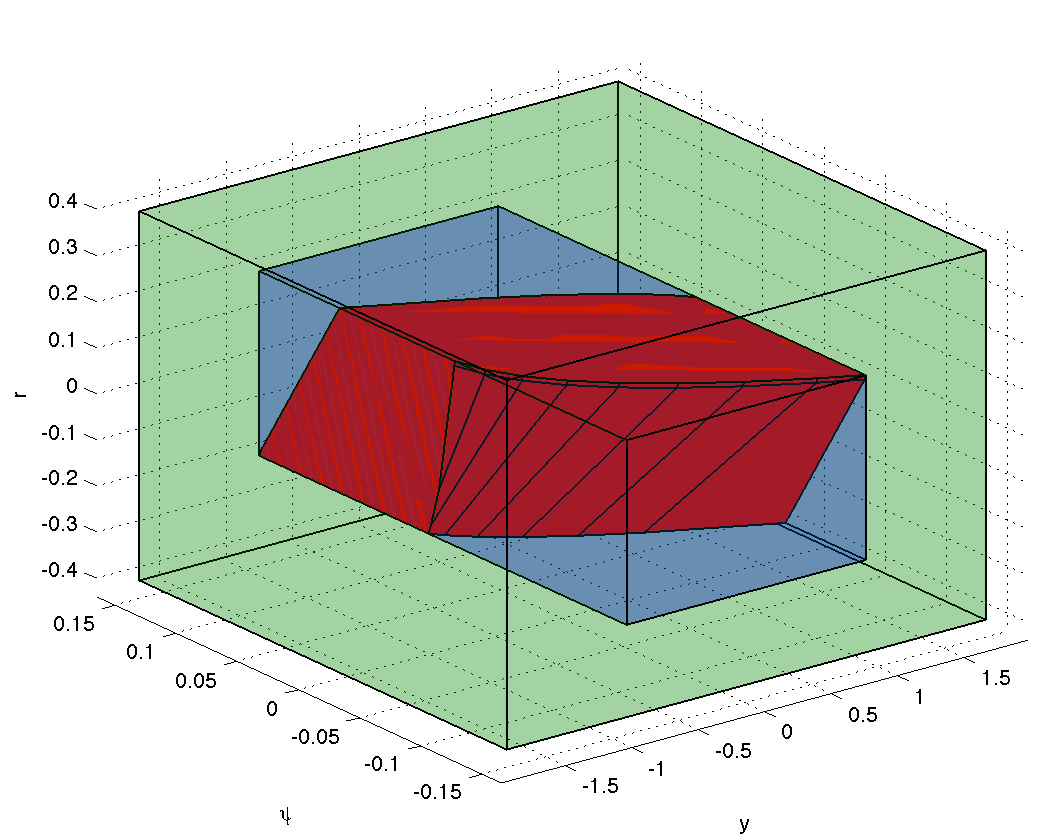
\includegraphics[width=0.4\columnwidth]{invariant}
		% This file was created by matlab2tikz v0.4.7 running on MATLAB 8.2.
% Copyright (c) 2008--2014, Nico Schlömer <nico.schloemer@gmail.com>
% All rights reserved.
% Minimal pgfplots version: 1.3
% 
\begin{tikzpicture}

\begin{axis}[%
width=\figurewidth,
height=\figureheight,
scale only axis,
xmin=0,
xmax=30,
ymin=-0.05,
ymax=0.05,
ylabel={$\psi$},
name=plot2,
axis x line*=bottom,
axis y line*=left
]
\addplot [color=blue,solid,forget plot]
  table[row sep=crcr]{0	0\\
0.1	-8.11922653108377e-11\\
0.2	-2.94274826471985e-10\\
0.3	-5.70599109401127e-10\\
0.4	-8.57046685346135e-10\\
0.5	-1.11645267556881e-09\\
0.6	-1.32502929540882e-09\\
0.7	-1.46982323270686e-09\\
0.8	-1.54639038646022e-09\\
0.9	-1.55670587213082e-09\\
1	-1.50731860379066e-09\\
1.1	-1.40775683539433e-09\\
1.2	-1.26918619845006e-09\\
1.3	-1.10331578030092e-09\\
1.4	-9.215416053197e-10\\
1.5	-7.34311210675931e-10\\
1.6	-5.50688306290393e-10\\
1.7	-3.78093033817029e-10\\
1.8	-2.22191190273808e-10\\
1.9	-8.69049355259197e-11\\
2	2.54821525094159e-11\\
2.1	1.14151446482498e-10\\
2.2	1.79530654256703e-10\\
2.3	2.230510367496e-10\\
2.4	2.4689812230643e-10\\
2.5	2.53770249125216e-10\\
2.6	2.46655935359844e-10\\
2.7	2.28637892469331e-10\\
2.8	2.02728577171907e-10\\
2.9	1.71739604727563e-10\\
3	1.38185173978418e-10\\
3.1	1.04217906866927e-10\\
3.2	7.15941827682171e-11\\
3.3	4.16651309986863e-11\\
3.4	1.53888985269601e-11\\
3.5	-6.64041181666412e-12\\
3.6	-2.41516870924157e-11\\
3.7	-3.71479214719673e-11\\
3.8	-4.58533642624988e-11\\
3.9	-5.06600209891922e-11\\
4	-5.20762313357276e-11\\
4.1	-5.06794293393911e-11\\
4.2	-4.70745870560919e-11\\
4.3	-4.18592803119233e-11\\
4.4	-3.55958134610909e-11\\
4.5	-2.87904126856009e-11\\
4.6	-2.18791508698328e-11\\
4.7	-1.52200029490366e-11\\
4.8	-9.09024632475928e-12\\
4.9	-3.68831021231078e-12\\
5	8.60868296384993e-13\\
5.1	4.49791464843484e-12\\
5.2	7.21939423898545e-12\\
5.3	9.06729166224723e-12\\
5.4	1.01182784894234e-11\\
5.5	1.04733352124429e-11\\
5.6	1.02481674685077e-11\\
5.7	9.5647336590538e-12\\
5.8	8.54408600063317e-12\\
5.9	7.30062416027075e-12\\
6	5.93777254861e-12\\
6.1	4.54502063215403e-12\\
6.2	3.19621049078042e-12\\
6.3	1.94891692214595e-12\\
6.4	8.44741617040131e-13\\
6.5	-8.96676979182726e-14\\
6.6	-8.41061618780288e-13\\
6.7	-1.40767554186092e-12\\
6.8	-1.79712026431867e-12\\
6.9	-2.02421730432732e-12\\
7	-2.10889539970274e-12\\
7.1	-2.07423936851874e-12\\
7.2	-1.94475760032252e-12\\
7.3	-1.74491116470999e-12\\
7.4	-1.4979264354358e-12\\
7.5	-1.22489509879741e-12\\
7.6	-9.44150626923299e-13\\
7.7	-6.70898863513267e-13\\
7.8	-4.17072226068556e-13\\
7.9	-1.91371873496799e-13\\
8	5.40141031669203e-16\\
8.1	1.55736803150716e-13\\
8.2	2.73646429325235e-13\\
8.3	3.55630361158349e-13\\
8.4	4.04546840681138e-13\\
8.5	4.24325022251693e-13\\
8.6	4.19568069680578e-13\\
8.7	3.95199164550798e-13\\
8.8	3.56159532808882e-13\\
8.9	3.07163309139897e-13\\
9	2.52510384703708e-13\\
9.1	1.9595529084143e-13\\
9.2	1.40627820387394e-13\\
9.3	8.89993886707929e-14\\
9.4	4.28880183054608e-14\\
9.5	3.49432082989194e-15\\
9.6	-2.85391884993143e-14\\
9.7	-5.30528190841832e-14\\
9.8	-7.02852097697565e-14\\
9.9	-8.07854979140885e-14\\
10	-8.53271235529993e-14\\
10.0137604070044	0.000614054579047492\\
10.0275208140088	0.00128969056296451\\
10.1	0.00484841859513103\\
10.1094087443329	0.00530872316761658\\
10.1188174886658	0.00576495593554063\\
10.1658612103304	0.00798504270673842\\
10.2	0.00953238122987587\\
10.3	0.01363006427895\\
10.4	0.0168826802735089\\
10.5	0.0191520106291827\\
10.6	0.0204021629209529\\
10.7	0.020668812807098\\
10.8	0.0200475444535412\\
10.9	0.0186854092399769\\
11	0.0167575524955817\\
11.1	0.0144474292229131\\
11.2	0.0119315906885171\\
11.3	0.00936874955351808\\
11.4	0.00689276486090274\\
11.5	0.00460895422618399\\
11.6	0.00258935348784601\\
11.7	0.000872722834569585\\
11.8	-0.000524728670855907\\
11.9	-0.00160350583377501\\
12	-0.00237780382095966\\
12.1	-0.00287258937294142\\
12.2	-0.00312064596669833\\
12.3	-0.00315972851254126\\
12.4	-0.00302995992190151\\
12.5	-0.00277156436998933\\
12.6	-0.00242299428789811\\
12.7	-0.00201947551423498\\
12.8	-0.00159196802777835\\
12.9	-0.00116651840079074\\
13	-0.000763964403792418\\
13.1	-0.000399941681446335\\
13.2	-8.51365656782984e-05\\
13.3	0.000174272754196068\\
13.4	0.000376043034750451\\
13.5	0.000521213240686861\\
13.6	0.000613418197219088\\
13.7	0.000658208119920864\\
13.8	0.000662406593005124\\
13.9	0.000633529826621865\\
14	0.000579283875649257\\
14.1	0.000507149327789809\\
14.2	0.000424056905803685\\
14.3	0.000336152357772449\\
14.4	0.000248644978949495\\
14.5	0.000165731119044214\\
14.6	9.0582028960938e-05\\
14.7	2.53843009753125e-05\\
14.8	-2.85791613306141e-05\\
14.9	-7.08195413263651e-05\\
15	-0.000101514274682286\\
15.1	-0.000121370816434714\\
15.2	-0.000131491114675507\\
15.3	-0.000133242393739105\\
15.4	-0.000128139630048468\\
15.5	-0.000117743253804682\\
15.6	-0.000103574173483018\\
15.7	-8.70469702464849e-05\\
15.8	-6.94210580895514e-05\\
15.9	-5.17687653894836e-05\\
16	-3.49586652091947e-05\\
16.1	-1.96520553750031e-05\\
16.2	-6.31024725714073e-06\\
16.3	4.7897590826923e-06\\
16.4	1.35335829273151e-05\\
16.5	1.99439650568632e-05\\
16.6	2.41534384984448e-05\\
16.7	2.63768545133834e-05\\
16.8	2.68851351427463e-05\\
16.9	2.5981301509983e-05\\
17	2.39795152135896e-05\\
17.1	2.11875818276354e-05\\
17.2	1.78931103648111e-05\\
17.3	1.4353306689144e-05\\
17.4	1.07882053407717e-05\\
17.5	7.37701344635041e-06\\
17.6	4.25715056328772e-06\\
17.7	1.5255160067206e-06\\
17.8	-7.58504180871018e-07\\
17.9	-2.5687702794815e-06\\
18	-3.90731154785927e-06\\
18.1	-4.79884175840963e-06\\
18.2	-5.28521369816765e-06\\
18.3	-5.42009554362819e-06\\
18.4	-5.26408707897436e-06\\
18.5	-4.88043054273421e-06\\
18.6	-4.33141221221924e-06\\
18.7	-3.67549867614996e-06\\
18.8	-2.96520740893803e-06\\
18.9	-2.24567541829736e-06\\
19	-1.55386252021772e-06\\
19.1	-9.18306884296458e-07\\
19.2	-3.59339224911901e-07\\
19.3	1.10342520371231e-07\\
19.4	4.84835049999351e-07\\
19.5	7.64019457494767e-07\\
19.6	9.52461203905629e-07\\
19.7	1.05829127235434e-06\\
19.8	1.09212682621428e-06\\
19.9	1.06607661058417e-06\\
19.9605807921388	1.02672971263974e-06\\
19.9893482375409	1.00295717234103e-06\\
20	-6.74949728054996e-05\\
20.0100988555802	-0.00101399150051312\\
20.0264373103001	-0.00261826984190363\\
20.1	-0.00983939558936009\\
20.2	-0.0192719072640704\\
20.3	-0.0275059673728831\\
20.4	-0.0340085394562876\\
20.5	-0.0385113162665394\\
20.6	-0.0409324133727168\\
20.7	-0.0413403921563173\\
20.8	-0.0399569880755265\\
20.9	-0.0370972929098225\\
21	-0.0331254805447789\\
21.1	-0.0284166011413822\\
21.2	-0.0233272723903758\\
21.3	-0.0181749791343795\\
21.4	-0.0132252703628319\\
21.5	-0.00868572216082228\\
21.6	-0.00470226024621395\\
21.7	-0.00136023147536542\\
21.8	0.00131226176933267\\
21.9	0.00333428972721868\\
22	0.004748870330059\\
22.1	0.0056164173463112\\
22.2	0.00600943157908607\\
22.3	0.00600734657530052\\
22.4	0.00569188130898003\\
22.5	0.00514303829922637\\
22.6	0.00443585256480859\\
22.7	0.00363792456179008\\
22.8	0.0028077266100698\\
22.9	0.00199364014010824\\
23	0.00123363370392003\\
23.1	0.000555485640447223\\
23.2	-2.25577867284188e-05\\
23.3	-0.000490798946614331\\
23.4	-0.000846888111874368\\
23.5	-0.00109450391757043\\
23.6	-0.0012420012115514\\
23.7	-0.00130109731725597\\
23.8	-0.00128564792826097\\
23.9	-0.00121055200895605\\
24	-0.00109081423037325\\
24.1	-0.000940781160305623\\
24.2	-0.000773556371320787\\
24.3	-0.00060058971134406\\
24.4	-0.000431428085179353\\
24.5	-0.000273609108256015\\
24.6	-0.000132674853282432\\
24.7	-1.22816131058815e-05\\
24.8	8.56184398777887e-05\\
24.9	0.000160546677292676\\
25	0.000213239376186438\\
25.1	0.000245379238140286\\
25.2	0.000259331956161445\\
25.3	0.000257899642901094\\
25.4	0.000244100308459425\\
25.5	0.000220979018302501\\
25.6	0.000191453850237237\\
25.7	0.000158197515905028\\
25.8	0.000123553609828142\\
25.9	8.94849583198706e-05\\
26	5.75504577925253e-05\\
26.1	2.89060925715187e-05\\
26.2	4.32550223935401e-06\\
26.3	-1.5764720247289e-05\\
26.4	-3.12395868783966e-05\\
26.5	-4.22241254479661e-05\\
26.6	-4.90394115179308e-05\\
26.7	-5.21493242750464e-05\\
26.8	-5.21104915086262e-05\\
26.9	-4.95272716108671e-05\\
27	-4.50130177500795e-05\\
27.1	-3.91583071415736e-05\\
27.2	-3.25063671634784e-05\\
27.3	-2.55355245792479e-05\\
27.4	-1.86481937590884e-05\\
27.5	-1.21656918754936e-05\\
27.6	-6.32801967319582e-06\\
27.7	-1.29766792380124e-06\\
27.8	2.83350765937696e-06\\
27.9	6.03526733097167e-06\\
28	8.32867638394659e-06\\
28.1	9.77525477731482e-06\\
28.2	1.04662220597865e-05\\
28.3	1.05123461177986e-05\\
28.4	1.00347773372869e-05\\
28.5	9.15712845637148e-06\\
28.6	7.99894956122152e-06\\
28.7	6.67065075458052e-06\\
28.8	5.26984408623537e-06\\
28.9	3.87901227761926e-06\\
29	2.56436450143962e-06\\
29.1	1.3757080925907e-06\\
29.2	3.47148064767023e-07\\
29.3	-5.01578231279225e-07\\
29.4	-1.16331820898364e-06\\
29.5	-1.64144599600194e-06\\
29.6	-1.94768267726972e-06\\
29.7	-2.09992487462657e-06\\
29.8	-2.12018641441149e-06\\
29.9	-2.03273225131636e-06\\
29.9695899823905	-1.92193131798056e-06\\
30	0.000193666027198354\\
};
\end{axis}

\begin{axis}[%
width=\figurewidth,
height=\figureheight,
scale only axis,
xmin=0,
xmax=30,
ymin=-1,
ymax=1,
ylabel={$y$},
at=(plot2.above north west),
anchor=below south west
]
\addplot [color=blue,solid,forget plot]
  table[row sep=crcr]{0	0\\
0.1	-8.11922653108378e-11\\
0.2	-6.22345811225611e-10\\
0.3	-1.91264499689916e-09\\
0.4	-4.05789244489903e-09\\
0.5	-7.02909455764372e-09\\
0.6	-1.07064855297974e-08\\
0.7	-1.49157931201043e-08\\
0.8	-1.94571964277945e-08\\
0.9	-2.41276582308046e-08\\
1	-2.87373521778653e-08\\
1.1	-3.31209291850559e-08\\
1.2	-3.7144379663253e-08\\
1.3	-4.07082439563006e-08\\
1.4	-4.37479006583683e-08\\
1.5	-4.62316218523658e-08\\
1.6	-4.81570280424602e-08\\
1.7	-4.95465069811747e-08\\
1.8	-5.04420835780727e-08\\
1.9	-5.09001465907383e-08\\
2	-5.09863555980291e-08\\
2.1	-5.07709721679858e-08\\
2.2	-5.03247849151831e-08\\
2.3	-4.9715731411967e-08\\
2.4	-4.90062621330795e-08\\
2.5	-4.82514436042183e-08\\
2.6	-4.74977599518466e-08\\
2.7	-4.67825438847491e-08\\
2.8	-4.61339491514712e-08\\
2.9	-4.55713657872049e-08\\
3	-4.51061758589867e-08\\
3.1	-4.47427496960268e-08\\
3.2	-4.4479589471788e-08\\
3.3	-4.43105372359172e-08\\
3.4	-4.4225976909999e-08\\
3.5	-4.42139733162574e-08\\
3.6	-4.42613051070704e-08\\
3.7	-4.43543617720641e-08\\
3.8	-4.44798871521294e-08\\
3.9	-4.46255626821258e-08\\
4	-4.47804326618321e-08\\
4.1	-4.49351810982285e-08\\
4.2	-4.50822750639139e-08\\
4.3	-4.52159931627253e-08\\
4.4	-4.53323597392513e-08\\
4.5	-4.54290061187781e-08\\
4.6	-4.55049796523066e-08\\
4.7	-4.55605199138197e-08\\
4.8	-4.55968192978328e-08\\
4.9	-4.56157827259647e-08\\
5	-4.56197983987336e-08\\
5.1	-4.56115287036417e-08\\
5.2	-4.55937276607014e-08\\
5.3	-4.55690887668236e-08\\
5.4	-4.55401248740666e-08\\
5.5	-4.55090798563096e-08\\
5.6	-4.54778703103373e-08\\
5.7	-4.54480544029221e-08\\
5.8	-4.54208241995072e-08\\
5.9	-4.53970173617802e-08\\
6	-4.5377143940118e-08\\
6.1	-4.53614240654039e-08\\
6.2	-4.5349832613442e-08\\
6.3	-4.53421473248804e-08\\
6.4	-4.53379973668285e-08\\
6.5	-4.53369098766911e-08\\
6.6	-4.53383525977034e-08\\
6.7	-4.5341771268158e-08\\
6.8	-4.53466209386741e-08\\
6.9	-4.53523908466393e-08\\
7	-4.53586228629378e-08\\
7.1	-4.53649238376667e-08\\
7.2	-4.53709724073243e-08\\
7.3	-4.53765209894159e-08\\
7.4	-4.53813937870204e-08\\
7.5	-4.53854816636962e-08\\
7.6	-4.53887347377288e-08\\
7.7	-4.53911534939206e-08\\
7.8	-4.53927791311287e-08\\
7.9	-4.53936837637557e-08\\
8	-4.5393960984349e-08\\
8.1	-4.53937171798874e-08\\
8.2	-4.5393063882387e-08\\
8.3	-4.53921113302243e-08\\
8.4	-4.53909633235886e-08\\
8.5	-4.53897133783923e-08\\
8.6	-4.53884421184727e-08\\
8.7	-4.53872157968882e-08\\
8.8	-4.53860858027661e-08\\
8.9	-4.53850889894546e-08\\
9	-4.53842486508936e-08\\
9.1	-4.53835759745144e-08\\
9.2	-4.53830718085259e-08\\
9.3	-4.53827285970246e-08\\
9.4	-4.53825323562007e-08\\
9.5	-4.53824645871586e-08\\
9.6	-4.53825040439052e-08\\
9.7	-4.53826282976775e-08\\
9.8	-4.53828150600751e-08\\
9.9	-4.5383043246334e-08\\
10	-4.53832937764988e-08\\
10.0137604070044	0.000113988452741948\\
10.0275208140088	0.0005069330725436\\
10.1	0.00718021040209756\\
10.1094087443329	0.00861379492966521\\
10.1188174886658	0.0101767319386806\\
10.1658612103304	0.0198914706264442\\
10.2	0.0288664005739314\\
10.3	0.0638018952095956\\
10.4	0.109809562719548\\
10.5	0.164117492751253\\
10.6	0.223701844051563\\
10.7	0.285543864442493\\
10.8	0.346821053516602\\
10.9	0.405080958398762\\
11	0.458359854276093\\
11.1	0.505236170299817\\
11.2	0.544831512132066\\
11.3	0.576772502048684\\
11.4	0.601125855532693\\
11.5	0.618317532039055\\
11.6	0.629041723865359\\
11.7	0.634155643979458\\
11.8	0.634597023939803\\
11.9	0.631326365001092\\
12	0.62528139817381\\
12.1	0.617340367970257\\
12.2	0.608294162107008\\
12.3	0.59882717817003\\
12.4	0.589506391205977\\
12.5	0.580777744440386\\
12.6	0.572968758767489\\
12.7	0.566296135831338\\
12.8	0.560877098177314\\
12.9	0.556743251035294\\
13	0.553855846789594\\
13.1	0.552121468893313\\
13.2	0.551407312079936\\
13.3	0.551555407195845\\
13.4	0.55239531086036\\
13.5	0.553754943814516\\
13.6	0.555469410478052\\
13.7	0.55738775880943\\
13.8	0.55937775018276\\
13.9	0.561328790156782\\
14	0.563153230911004\\
14.1	0.564786295111131\\
14.2	0.566184890153367\\
14.3	0.567325584207491\\
14.4	0.568202004291332\\
14.5	0.568821894899983\\
14.6	0.569204046538715\\
14.7	0.569375269711571\\
14.8	0.569367554026461\\
14.9	0.569215516093975\\
15	0.56895420569878\\
15.1	0.568617311025397\\
15.2	0.568235772822881\\
15.3	0.567836797241628\\
15.4	0.567443239822103\\
15.5	0.567073319879205\\
15.6	0.566740616127064\\
15.7	0.566454290020731\\
15.8	0.566219482379083\\
15.9	0.566037830779593\\
16	0.565908059343153\\
16.1	0.565826598232834\\
16.2	0.565788196893488\\
16.3	0.565786502240563\\
16.4	0.565814580223768\\
16.5	0.565865366084228\\
16.6	0.565932034917361\\
16.7	0.56600828965451\\
16.8	0.566088568166993\\
16.9	0.566168174825946\\
17	0.56624334452641\\
17.1	0.566311248956128\\
17.2	0.566369955844457\\
17.3	0.56641835217409\\
17.4	0.566456042001205\\
17.5	0.56648322873631\\
17.6	0.566500590614509\\
17.7	0.566509156748277\\
17.8	0.566510189713884\\
17.9	0.566505079165322\\
18	0.566495249571062\\
18.1	0.56648208388643\\
18.2	0.566466863848406\\
18.3	0.566450726635279\\
18.4	0.566434636882449\\
18.5	0.566419372487375\\
18.6	0.566405522261817\\
18.7	0.566393493281285\\
18.8	0.566383525718351\\
18.9	0.566375713003575\\
19	0.566370025309434\\
19.1	0.566366334573353\\
19.2	0.566364439541696\\
19.3	0.566364089605778\\
19.4	0.566365006494991\\
19.5	0.56636690317568\\
19.6	0.566369499565599\\
19.7	0.566372534904123\\
19.8	0.566375776812514\\
19.9	0.566379027233886\\
19.9605807921388	0.566380931196237\\
19.9893482375409	0.566381807265479\\
20	0.566382126236082\\
20.0100988555802	0.566225144304234\\
20.0264373103001	0.565334954583245\\
20.1	0.551588056163345\\
20.2	0.507689355078309\\
20.3	0.437127397315184\\
20.4	0.344369915836634\\
20.5	0.235070466823728\\
20.6	0.115383622319823\\
20.7	-0.00850310112939186\\
20.8	-0.130854825505024\\
20.9	-0.246753431860216\\
21	-0.352310167653342\\
21.1	-0.444753362138088\\
21.2	-0.522414873788062\\
21.3	-0.584641685010991\\
21.4	-0.631657442445099\\
21.5	-0.664396137533923\\
21.6	-0.684323320370016\\
21.7	-0.693248921630284\\
21.8	-0.693154669729446\\
21.9	-0.686027356266407\\
22	-0.673758749406503\\
22.1	-0.65808414481232\\
22.2	-0.640538131879383\\
22.3	-0.622426175687266\\
22.4	-0.604810937232511\\
22.5	-0.588511600941238\\
22.6	-0.574114097718101\\
22.7	-0.561989902311225\\
22.8	-0.552321069467567\\
22.9	-0.54512923171826\\
23	-0.540306502414787\\
23.1	-0.537646500612299\\
23.2	-0.536874027267137\\
23.3	-0.537672251437246\\
23.4	-0.539706594112297\\
23.5	-0.542644809150187\\
23.6	-0.546173036442427\\
23.7	-0.550007842030949\\
23.8	-0.553904440636819\\
23.9	-0.557661430918173\\
24	-0.56112247649106\\
24.1	-0.564175432511554\\
24.2	-0.566749449450244\\
24.3	-0.56881058595625\\
24.4	-0.57035643586435\\
24.5	-0.571410227355509\\
24.6	-0.572014789180624\\
24.7	-0.572226708245357\\
24.8	-0.572110930261419\\
24.9	-0.571735984228069\\
25	-0.571169945576751\\
25.1	-0.570477194145341\\
25.2	-0.569715973137887\\
25.3	-0.568936715821924\\
25.4	-0.568181074545866\\
25.5	-0.567481564829261\\
25.6	-0.566861724211731\\
25.7	-0.566336679647385\\
25.8	-0.565914017590953\\
25.9	-0.565594856372638\\
26	-0.565375029765342\\
26.1	-0.565246302619204\\
26.2	-0.565197552948924\\
26.3	-0.565215868967892\\
26.4	-0.565287524021536\\
26.5	-0.565398804962045\\
26.6	-0.565536681346025\\
26.7	-0.565689313130931\\
26.8	-0.565846402900772\\
26.9	-0.565999405105096\\
27	-0.566141609449314\\
27.1	-0.566268118420896\\
27.2	-0.5663757403063\\
27.3	-0.566462819114791\\
27.4	-0.566529021817705\\
27.5	-0.566575101497198\\
27.6	-0.56660265261971\\
27.7	-0.566613871931067\\
27.8	-0.566611335610728\\
27.9	-0.566597800489512\\
28	-0.566576034462092\\
28.1	-0.566548678813032\\
28.2	-0.566518143091405\\
28.3	-0.566486531453233\\
28.4	-0.566455598056668\\
28.5	-0.566426728134206\\
28.6	-0.566400940754884\\
28.7	-0.566378908990236\\
28.8	-0.566360993165853\\
28.9	-0.566347283065936\\
29	-0.566337645310651\\
29.1	-0.566331772596181\\
29.2	-0.566329232029567\\
29.3	-0.56632951036443\\
29.4	-0.566332054515255\\
29.5	-0.566336306269576\\
29.6	-0.566341730608368\\
29.7	-0.566347837470818\\
29.8	-0.566354197152053\\
29.9	-0.566360449798163\\
29.9695899823905	-0.566364583627999\\
30	-0.566366310671168\\
};
\end{axis}

\begin{axis}[%
width=\figurewidth,
height=\figureheight,
scale only axis,
xmin=0,
xmax=30,
ymin=-0.1,
ymax=0.3,
ylabel={$r$},
at=(plot2.below south west),
anchor=above north west,
axis x line*=bottom,
axis y line*=left
]
\addplot [color=red,solid,forget plot]
  table[row sep=crcr]{0	0\\
0.1	0\\
0.2	0\\
0.3	0\\
0.4	0\\
0.5	0\\
0.6	0\\
0.7	0\\
0.8	0\\
0.9	0\\
1	0\\
1.1	0\\
1.2	0\\
1.3	0\\
1.4	0\\
1.5	0\\
1.6	0\\
1.7	0\\
1.8	0\\
1.9	0\\
2	0\\
2.1	0\\
2.2	0\\
2.3	0\\
2.4	0\\
2.5	0\\
2.6	0\\
2.7	0\\
2.8	0\\
2.9	0\\
3	0\\
3.1	0\\
3.2	0\\
3.3	0\\
3.4	0\\
3.5	0\\
3.6	0\\
3.7	0\\
3.8	0\\
3.9	0\\
4	0\\
4.1	0\\
4.2	0\\
4.3	0\\
4.4	0\\
4.5	0\\
4.6	0\\
4.7	0\\
4.8	0\\
4.9	0\\
5	0\\
5.1	0\\
5.2	0\\
5.3	0\\
5.4	0\\
5.5	0\\
5.6	0\\
5.7	0\\
5.8	0\\
5.9	0\\
6	0\\
6.1	0\\
6.2	0\\
6.3	0\\
6.4	0\\
6.5	0\\
6.6	0\\
6.7	0\\
6.8	0\\
6.9	0\\
7	0\\
7.1	0\\
7.2	0\\
7.3	0\\
7.4	0\\
7.5	0\\
7.6	0\\
7.7	0\\
7.8	0\\
7.9	0\\
8	0\\
8.1	0\\
8.2	0\\
8.3	0\\
8.4	0\\
8.5	0\\
8.6	0\\
8.7	0\\
8.8	0\\
8.9	0\\
9	0\\
9.1	0\\
9.2	0\\
9.3	0\\
9.4	0\\
9.5	0\\
9.6	0\\
9.7	0\\
9.8	0\\
9.9	0\\
10	0\\
10.0137604070044	0.0491\\
10.0275208140088	0.0491\\
10.1	0.0491\\
10.1094087443329	0.0491\\
10.1188174886658	0.0491\\
10.1658612103304	0.0491\\
10.2	0.0491\\
10.3	0.0491\\
10.4	0.0491\\
10.5	0.0491\\
10.6	0.0491\\
10.7	0.0491\\
10.8	0.0491\\
10.9	0.0491\\
11	0.0491\\
11.1	0.0491\\
11.2	0.0491\\
11.3	0.0491\\
11.4	0.0491\\
11.5	0.0491\\
11.6	0.0491\\
11.7	0.0491\\
11.8	0.0491\\
11.9	0.0491\\
12	0.0491\\
12.1	0.0491\\
12.2	0.0491\\
12.3	0.0491\\
12.4	0.0491\\
12.5	0.0491\\
12.6	0.0491\\
12.7	0.0491\\
12.8	0.0491\\
12.9	0.0491\\
13	0.0491\\
13.1	0.0491\\
13.2	0.0491\\
13.3	0.0491\\
13.4	0.0491\\
13.5	0.0491\\
13.6	0.0491\\
13.7	0.0491\\
13.8	0.0491\\
13.9	0.0491\\
14	0.0491\\
14.1	0.0491\\
14.2	0.0491\\
14.3	0.0491\\
14.4	0.0491\\
14.5	0.0491\\
14.6	0.0491\\
14.7	0.0491\\
14.8	0.0491\\
14.9	0.0491\\
15	0.0491\\
15.1	0.0491\\
15.2	0.0491\\
15.3	0.0491\\
15.4	0.0491\\
15.5	0.0491\\
15.6	0.0491\\
15.7	0.0491\\
15.8	0.0491\\
15.9	0.0491\\
16	0.0491\\
16.1	0.0491\\
16.2	0.0491\\
16.3	0.0491\\
16.4	0.0491\\
16.5	0.0491\\
16.6	0.0491\\
16.7	0.0491\\
16.8	0.0491\\
16.9	0.0491\\
17	0.0491\\
17.1	0.0491\\
17.2	0.0491\\
17.3	0.0491\\
17.4	0.0491\\
17.5	0.0491\\
17.6	0.0491\\
17.7	0.0491\\
17.8	0.0491\\
17.9	0.0491\\
18	0.0491\\
18.1	0.0491\\
18.2	0.0491\\
18.3	0.0491\\
18.4	0.0491\\
18.5	0.0491\\
18.6	0.0491\\
18.7	0.0491\\
18.8	0.0491\\
18.9	0.0491\\
19	0.0491\\
19.1	0.0491\\
19.2	0.0491\\
19.3	0.0491\\
19.4	0.0491\\
19.5	0.0491\\
19.6	0.0491\\
19.7	0.0491\\
19.8	0.0491\\
19.9	0.0491\\
19.9605807921388	0.0491\\
19.9893482375409	0.0491\\
20	0\\
20.0100988555802	-0.0491\\
20.0264373103001	-0.0491\\
20.1	-0.0491\\
20.2	-0.0491\\
20.3	-0.0491\\
20.4	-0.0491\\
20.5	-0.0491\\
20.6	-0.0491\\
20.7	-0.0491\\
20.8	-0.0491\\
20.9	-0.0491\\
21	-0.0491\\
21.1	-0.0491\\
21.2	-0.0491\\
21.3	-0.0491\\
21.4	-0.0491\\
21.5	-0.0491\\
21.6	-0.0491\\
21.7	-0.0491\\
21.8	-0.0491\\
21.9	-0.0491\\
22	-0.0491\\
22.1	-0.0491\\
22.2	-0.0491\\
22.3	-0.0491\\
22.4	-0.0491\\
22.5	-0.0491\\
22.6	-0.0491\\
22.7	-0.0491\\
22.8	-0.0491\\
22.9	-0.0491\\
23	-0.0491\\
23.1	-0.0491\\
23.2	-0.0491\\
23.3	-0.0491\\
23.4	-0.0491\\
23.5	-0.0491\\
23.6	-0.0491\\
23.7	-0.0491\\
23.8	-0.0491\\
23.9	-0.0491\\
24	-0.0491\\
24.1	-0.0491\\
24.2	-0.0491\\
24.3	-0.0491\\
24.4	-0.0491\\
24.5	-0.0491\\
24.6	-0.0491\\
24.7	-0.0491\\
24.8	-0.0491\\
24.9	-0.0491\\
25	-0.0491\\
25.1	-0.0491\\
25.2	-0.0491\\
25.3	-0.0491\\
25.4	-0.0491\\
25.5	-0.0491\\
25.6	-0.0491\\
25.7	-0.0491\\
25.8	-0.0491\\
25.9	-0.0491\\
26	-0.0491\\
26.1	-0.0491\\
26.2	-0.0491\\
26.3	-0.0491\\
26.4	-0.0491\\
26.5	-0.0491\\
26.6	-0.0491\\
26.7	-0.0491\\
26.8	-0.0491\\
26.9	-0.0491\\
27	-0.0491\\
27.1	-0.0491\\
27.2	-0.0491\\
27.3	-0.0491\\
27.4	-0.0491\\
27.5	-0.0491\\
27.6	-0.0491\\
27.7	-0.0491\\
27.8	-0.0491\\
27.9	-0.0491\\
28	-0.0491\\
28.1	-0.0491\\
28.2	-0.0491\\
28.3	-0.0491\\
28.4	-0.0491\\
28.5	-0.0491\\
28.6	-0.0491\\
28.7	-0.0491\\
28.8	-0.0491\\
28.9	-0.0491\\
29	-0.0491\\
29.1	-0.0491\\
29.2	-0.0491\\
29.3	-0.0491\\
29.4	-0.0491\\
29.5	-0.0491\\
29.6	-0.0491\\
29.7	-0.0491\\
29.8	-0.0491\\
29.9	-0.0491\\
29.9695899823905	-0.0491\\
30	0\\
};
\addplot [color=blue,solid,forget plot]
  table[row sep=crcr]{0	0\\
0.1	-1.62384530621676e-09\\
0.2	-2.56982513885346e-09\\
0.3	-2.9019129764928e-09\\
0.4	-2.78777893891346e-09\\
0.5	-2.37425311034735e-09\\
0.6	-1.78196843166073e-09\\
0.7	-1.10717085431314e-09\\
0.8	-4.2400930397745e-10\\
0.9	2.1306091209435e-10\\
1	7.66791843802708e-10\\
1.1	1.21461380305122e-09\\
1.2	1.54611979988266e-09\\
1.3	1.76062603629072e-09\\
1.4	1.86486883311251e-09\\
1.5	1.87089053142448e-09\\
1.6	1.7941555655891e-09\\
1.7	1.65192486674047e-09\\
1.8	1.46190340497729e-09\\
1.9	1.24116306611726e-09\\
2	1.00533191335327e-09\\
2.1	7.68031671638409e-10\\
2.2	5.4053820739258e-10\\
2.3	3.31634933395339e-10\\
2.4	1.47626322198127e-10\\
2.5	-7.52211844916736e-12\\
2.6	-1.31950253290517e-10\\
2.7	-2.25606828081685e-10\\
2.8	-2.89917677867181e-10\\
2.9	-3.27442428719796e-10\\
3	-3.41539314335309e-10\\
3.1	-3.36053430746415e-10\\
3.2	-3.15039565694807e-10\\
3.3	-2.82526832468088e-10\\
3.4	-2.42328843792384e-10\\
3.5	-1.97900171487145e-10\\
3.6	-1.5223739111503e-10\\
3.7	-1.07821124509785e-10\\
3.8	-6.65941535546279e-11\\
3.9	-2.99698350060208e-11\\
4	1.13534129054239e-12\\
4.1	2.625122849028e-11\\
4.2	4.52914101919645e-11\\
4.3	5.84838549218295e-11\\
4.4	6.62995006535585e-11\\
4.5	6.93826462158838e-11\\
4.6	6.84861994741817e-11\\
4.7	6.44140165506907e-11\\
4.8	5.79717874777038e-11\\
4.9	4.99272362643543e-11\\
5	4.09797961955214e-11\\
5.1	3.17394300020004e-11\\
5.2	2.27138814253823e-11\\
5.3	1.4303368027481e-11\\
5.4	6.80155148247289e-12\\
5.5	4.01536091264669e-13\\
5.6	-4.79435838212933e-12\\
5.7	-8.76225065368174e-12\\
5.8	-1.15428742854209e-11\\
5.9	-1.32272359268889e-11\\
6	-1.39425554994846e-11\\
6.1	-1.38391220008252e-11\\
6.2	-1.30785342036062e-11\\
6.3	-1.18236359222703e-11\\
6.4	-1.02303134362168e-11\\
6.5	-8.44120201255207e-12\\
6.6	-6.58124323053848e-12\\
6.7	-4.75495700968715e-12\\
6.8	-3.04523384239983e-12\\
6.9	-1.51341554309328e-12\\
7	-2.00415213892061e-13\\
7.1	8.71378783466446e-13\\
7.2	1.6956560386774e-12\\
7.3	2.27941884316326e-12\\
7.4	2.64009477855571e-12\\
7.5	2.80269111708154e-12\\
7.6	2.79712287316286e-12\\
7.7	2.65581100158589e-12\\
7.8	2.41161773576783e-12\\
7.9	2.09615495262284e-12\\
8	1.73847694177762e-12\\
8.1	1.36414834456637e-12\\
8.2	9.94660846332281e-13\\
8.3	6.47161013638343e-13\\
8.4	3.344416533772e-13\\
8.5	6.51488292840089e-14\\
8.6	-1.55848313190869e-13\\
8.7	-3.26973536359827e-13\\
8.8	-4.4939133007026e-13\\
8.9	-5.26425858525353e-13\\
9	-5.62985443829235e-13\\
9.1	-5.65019779508147e-13\\
9.2	-5.39029712025691e-13\\
9.3	-4.9164392815298e-13\\
9.4	-4.2927045850378e-13\\
9.5	-3.57825412339134e-13\\
9.6	-2.82537408117159e-13\\
9.7	-2.0782361378229e-13\\
9.8	-1.37228368590926e-13\\
9.9	-7.34172146084666e-14\\
10	-1.8214437033076e-14\\
10.0137604070044	-1.19478980935457e-14\\
10.0275208140088	-5.8036709334889e-15\\
10.1	2.65593676715862e-14\\
10.1094087443329	-0.000393323105652787\\
10.1188174886658	-0.00082609122193077\\
10.1658612103304	-0.00298993180332068\\
10.2	-0.00456019231572906\\
10.3	-0.0119677425535038\\
10.4	-0.0213497041539368\\
10.5	-0.0315263606220314\\
10.6	-0.0416599937327086\\
10.7	-0.0511428026618412\\
10.8	-0.0593623113982453\\
10.9	-0.0659264403291893\\
11	-0.0706628369933811\\
11.1	-0.0735733508576698\\
11.2	-0.0747902483171021\\
11.3	-0.0745342208930131\\
11.4	-0.0730784256800208\\
11.5	-0.070717777886746\\
11.6	-0.0678293294182144\\
11.7	-0.0646818054803717\\
11.8	-0.0614621441945055\\
11.9	-0.0583218700212347\\
12	-0.0553834871813748\\
12.1	-0.052739836189547\\
12.2	-0.0504544563081405\\
12.3	-0.0485634159927314\\
12.4	-0.047078287129696\\
12.5	-0.0459898683991183\\
12.6	-0.0452723047371501\\
12.7	-0.0448873043047814\\
12.8	-0.0447882116197382\\
12.9	-0.0449237525087443\\
13	-0.0452413207741734\\
13.1	-0.0456897260148116\\
13.2	-0.0462213655273006\\
13.3	-0.0467938197988688\\
13.4	-0.0473709004112481\\
13.5	-0.0479231973868444\\
13.6	-0.0484282122472045\\
13.7	-0.0488701099036248\\
13.8	-0.0492392096042514\\
13.9	-0.0495312730505288\\
14	-0.0497466640424109\\
14.1	-0.0498894453327554\\
14.2	-0.0499664684964771\\
14.3	-0.049986502367031\\
14.4	-0.0499594350738026\\
14.5	-0.0498955744707279\\
14.6	-0.0498050622324983\\
14.7	-0.0496974084421774\\
14.8	-0.049581146317633\\
14.9	-0.0494636046107615\\
15	-0.0493507675526612\\
15.1	-0.0492472500187035\\
15.2	-0.0491563304218345\\
15.3	-0.0490800449844573\\
15.4	-0.0490193254198734\\
15.5	-0.0489741643904854\\
15.6	-0.0489437952952349\\
15.7	-0.0489268748444177\\
15.8	-0.0489216589538643\\
15.9	-0.0489261646286284\\
16	-0.0489383125938034\\
16.1	-0.0489560473746637\\
16.2	-0.0489774332622805\\
16.3	-0.0490007260795864\\
16.4	-0.0490244218630396\\
16.5	-0.049047284491161\\
16.6	-0.0490683549328025\\
16.7	-0.0490869451761602\\
16.8	-0.0491026200637576\\
16.9	-0.0491151702336631\\
17	-0.0491245791904737\\
17.1	-0.0491309872387465\\
17.2	-0.0491346546426426\\
17.3	-0.0491359259615299\\
17.4	-0.049135197081051\\
17.5	-0.0491328860368463\\
17.6	-0.0491294083328715\\
17.7	-0.0491251571022272\\
17.8	-0.0491204881550568\\
17.9	-0.0491157097105217\\
18	-0.0491110764195715\\
18.1	-0.049106787150548\\
18.2	-0.0491029859265545\\
18.3	-0.0490997653661891\\
18.4	-0.0490971719807601\\
18.5	-0.0490952127139704\\
18.6	-0.0490938621666722\\
18.7	-0.0490930700223493\\
18.8	-0.0490927682717612\\
18.9	-0.0490928779217792\\
19	-0.0490933149588859\\
19.1	-0.0490939954181478\\
19.2	-0.0490948394807429\\
19.3	-0.0490957745853474\\
19.4	-0.0490967375897254\\
19.5	-0.0490976760583746\\
19.6	-0.0490985487803272\\
19.7	-0.0490993256389529\\
19.8	-0.0490999869640176\\
19.9	-0.0491005224966669\\
19.9605807921388	-0.0491007694211242\\
19.9893482375409	-0.0491008833179332\\
20	-0.0491009254906649\\
20.0100988555802	-0.0490953238915918\\
20.0264373103001	-0.0490853459928587\\
20.1	-0.0490404212382876\\
20.2	-0.0405660738373393\\
20.3	-0.025320701304647\\
20.4	-0.00620190071981568\\
20.5	0.0144690456460339\\
20.6	0.0353141774153078\\
20.7	0.054565934935014\\
20.8	0.0710396206207114\\
20.9	0.0840314246858735\\
21	0.0932597774414358\\
21.1	0.0987805985121892\\
21.2	0.100898530381745\\
21.3	0.100084089997604\\
21.4	0.0968987122474094\\
21.5	0.0919351185662022\\
21.6	0.085836000243047\\
21.7	0.0791561785044741\\
21.8	0.072501012568649\\
21.9	0.0661714672330136\\
22	0.0603698918934955\\
22.1	0.0552438015152278\\
22.2	0.0508873769688907\\
22.3	0.0473455015689265\\
22.4	0.0446195389367532\\
22.5	0.0426744567777358\\
22.6	0.0414466563370838\\
22.7	0.0408517533369504\\
22.8	0.0407922696812227\\
22.9	0.0411644822872263\\
23	0.0418643935924598\\
23.1	0.0427926347791445\\
23.2	0.0438582708412469\\
23.3	0.0449815010925071\\
23.4	0.0460953099317408\\
23.5	0.0471462055781819\\
23.6	0.0480941416927738\\
23.7	0.048911849515529\\
23.8	0.049583725417649\\
23.9	0.0501043718134783\\
24	0.050476917307969\\
24.1	0.0507112318989239\\
24.2	0.0508221429746816\\
24.3	0.0508277443580303\\
24.4	0.0507478626562663\\
24.5	0.0506027386983928\\
24.6	0.0504119459060242\\
24.7	0.0501935520814613\\
24.8	0.0499635190858796\\
24.9	0.0497353231504941\\
25	0.0495197710004604\\
25.1	0.0493249843676893\\
25.2	0.0491565126503963\\
25.3	0.0490175560916486\\
25.4	0.0489092597474727\\
25.5	0.0488310507491811\\
25.6	0.0487809948524407\\
25.7	0.0487561512920619\\
25.8	0.0487529089648239\\
25.9	0.0487672911088803\\
26	0.0487952196395914\\
26.1	0.0488327339618272\\
26.2	0.0488761630737491\\
26.3	0.0489222477653778\\
26.4	0.0489682222601679\\
26.5	0.0490118554395746\\
26.6	0.0490514578237774\\
26.7	0.0490858606901638\\
26.8	0.0491143737593799\\
26.9	0.0491367272963834\\
27	0.0491530049468748\\
27.1	0.0491635720123209\\
27.2	0.0491690036461126\\
27.3	0.0491700165091958\\
27.4	0.0491674065724802\\
27.5	0.0491619949389031\\
27.6	0.0491545828058234\\
27.7	0.0491459160251865\\
27.8	0.0491366591603837\\
27.9	0.0491273784923623\\
28	0.0491185330937179\\
28.1	0.0491104728629773\\
28.2	0.0491034422825328\\
28.3	0.0490975886202317\\
28.4	0.0490929733221893\\
28.5	0.0490895854279965\\
28.6	0.0490873559642828\\
28.7	0.0490861724245816\\
28.8	0.0490858926099689\\
28.9	0.0490863572751023\\
29	0.0490874011890439\\
29.1	0.0490888623726018\\
29.2	0.0490905894087846\\
29.3	0.0490924468370889\\
29.4	0.0490943187341085\\
29.5	0.049096110652156\\
29.6	0.0490977501351434\\
29.7	0.0490991860586958\\
29.8	0.0491003870518034\\
29.9	0.0491013392530631\\
29.9695899823905	0.0491018294349302\\
30	0.0491020367757445\\
};
\end{axis}
\end{tikzpicture}%
	\end{center}
	\caption{Car states in simulation. Yellow line is $r_{road}$.}
	\label{fig:invariant}
\end{figure}
\setlength\figurewidth{0.8\columnwidth} 
\setlength\figureheight{0.4 \columnwidth} 

\begin{figure}[h]
	\begin{center}
		% 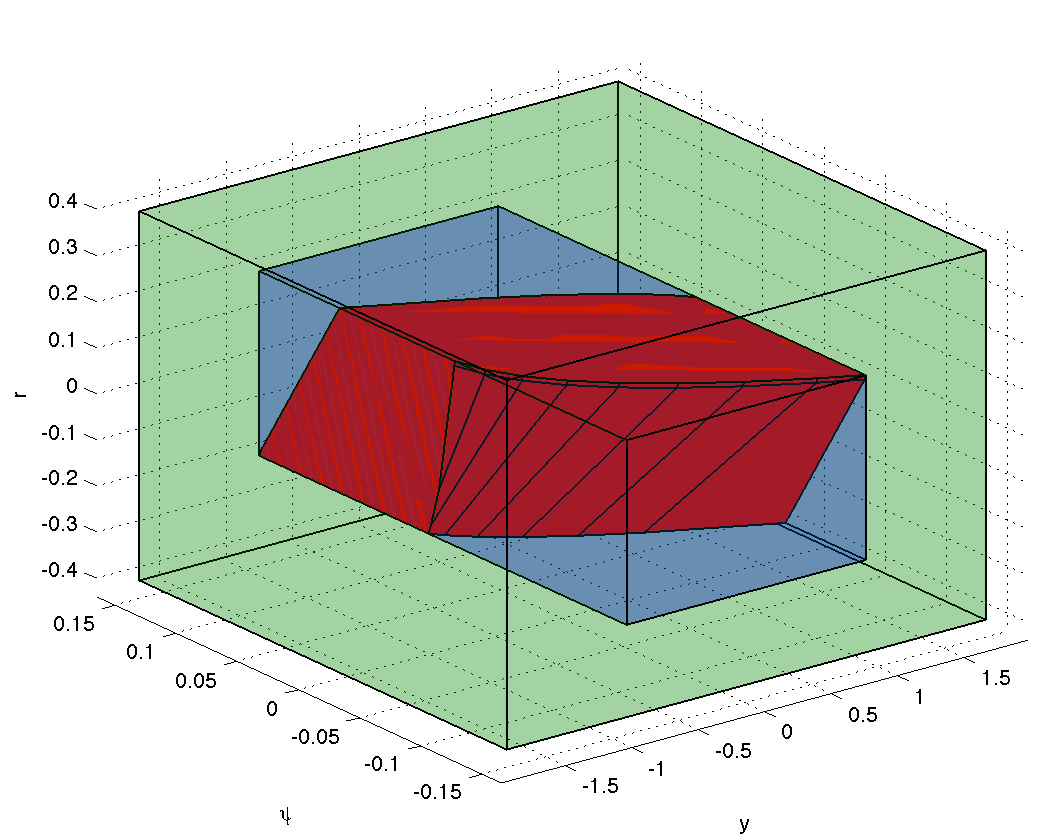
\includegraphics[width=0.4\columnwidth]{invariant}
		% This file was created by matlab2tikz v0.4.7 running on MATLAB 8.2.
% Copyright (c) 2008--2014, Nico Schlömer <nico.schloemer@gmail.com>
% All rights reserved.
% Minimal pgfplots version: 1.3
% 
\begin{tikzpicture}

\begin{axis}[%
width=\figurewidth,
height=\figureheight,
scale only axis,
xmin=0,
xmax=30,
ymin=-0.2,
ymax=0.15,
ylabel={$\delta_f$},
axis x line*=bottom,
axis y line*=left
]
\addplot [color=red,solid,forget plot]
  table[row sep=crcr]{0	-1.07232454548144e-09\\
0.05	-0.124654863151455\\
0.1	-0.139201079402639\\
0.15	-0.0759764873456075\\
0.2	0.0168832533420676\\
0.25	0.0897873237236122\\
0.3	0.111839955155193\\
0.35	0.0813500609018836\\
0.4	0.021638170207335\\
0.45	-0.0340671530538241\\
0.5	-0.0599356515888013\\
0.55	-0.0485619355328274\\
0.6	-0.011510841045794\\
0.65	0.0292047639332634\\
0.7	0.0532374835956317\\
0.75	0.0513054423578992\\
0.8	0.0278598334929474\\
0.85	-0.0031742919260469\\
0.9	-0.0264690427806885\\
0.95	-0.0327518732142345\\
1	-0.0222186007755997\\
1.05	-0.00292806159433704\\
1.1	0.0142654931683359\\
1.15	0.0212947795657196\\
1.2	0.0162535480720353\\
1.25	0.0033167034442891\\
1.3	-0.0102067780361014\\
1.35	-0.017837653049327\\
1.4	-0.0168691338259113\\
1.45	-0.0090575305857093\\
1.5	0.000908919319529633\\
1.55	0.00808598285038881\\
1.6	0.00964624954997265\\
1.65	0.00587424567938105\\
1.7	-0.000468225321844175\\
1.75	-0.00584736826059661\\
1.8	-0.00775622987760246\\
1.85	-0.00574094975485868\\
1.9	-0.00129150165517451\\
1.95	0.00317105227868263\\
2	0.00558791964872439\\
2.05	0.00517983784882924\\
2.1	0.00261368296534284\\
2.15	-0.000541344890873519\\
2.2	-0.00269793602412957\\
2.25	-0.00300289810918341\\
2.3	-0.00162245865094822\\
2.35	0.000500158424683009\\
2.4	0.0022162976012215\\
2.45	0.00274977002420648\\
2.5	0.00200654537130887\\
2.55	0.000512228313061371\\
2.6	-0.000934011616449412\\
2.65	-0.00168026475617156\\
2.7	-0.00150642986824645\\
2.75	-0.000659445020938763\\
2.8	0.000337909575105051\\
2.85	0.000978227869783182\\
2.9	0.00100704207806349\\
2.95	0.00050285297839894\\
3	-0.000213209375852655\\
3.05	-0.000768265841213187\\
3.1	-0.000922787738229165\\
3.15	-0.000663212734561972\\
3.2	-0.000172910633852355\\
3.25	0.000285462195344355\\
3.3	0.000506487431958519\\
3.35	0.000429789269782559\\
3.4	0.000145305705469285\\
3.45	-0.000173361882226361\\
3.5	-0.000364559470164538\\
3.55	-0.000353307342294433\\
3.6	-0.000173097604202015\\
3.65	6.71454259158085e-05\\
3.7	0.000246594086043564\\
3.75	0.000291623583602571\\
3.8	0.000203219257011813\\
3.85	4.47407963501891e-05\\
3.9	-9.78779384672544e-05\\
3.95	-0.000160287101173384\\
4	-0.000126651931739559\\
4.05	-2.93506152496192e-05\\
4.1	7.40911305502838e-05\\
4.15	0.000132296450152386\\
4.2	0.000123445052255258\\
4.25	6.09658040672602e-05\\
4.3	-1.83677758849413e-05\\
4.35	-7.55114486855858e-05\\
4.4	-8.79640499192217e-05\\
4.45	-5.77754587997979e-05\\
4.5	-6.67342566541878e-06\\
4.55	3.73407149789494e-05\\
4.6	5.42307739738913e-05\\
4.65	4.01292904708376e-05\\
4.7	6.5831412600905e-06\\
4.75	-2.73783075721147e-05\\
4.8	-4.54580424902099e-05\\
4.85	-4.13915538161766e-05\\
4.9	-2.0339366577468e-05\\
4.95	5.34984256027996e-06\\
5	2.31072019345171e-05\\
5.05	2.61118389307065e-05\\
5.1	1.55937899394584e-05\\
5.15	-1.03623394536087e-06\\
5.2	-1.46826195242297e-05\\
5.25	-1.91418135296741e-05\\
5.3	-1.35817285751871e-05\\
5.35	-2.0834826075117e-06\\
5.4	9.07096575089111e-06\\
5.45	1.47234707623713e-05\\
5.5	1.310571877341e-05\\
5.55	6.14198440192655e-06\\
5.6	-2.04324265465869e-06\\
5.65	-7.42174271283911e-06\\
5.7	-7.94790256926696e-06\\
5.75	-4.20749144821237e-06\\
5.8	1.28153115847309e-06\\
5.85	5.57116274685004e-06\\
5.9	6.75001097416263e-06\\
5.95	4.68594986782505e-06\\
6	8.08248285661262e-07\\
6.05	-2.81521065177817e-06\\
6.1	-4.55696353820657e-06\\
6.15	-3.92974262889277e-06\\
6.2	-1.63597623910649e-06\\
6.25	9.53238379437362e-07\\
6.3	2.55260242526271e-06\\
6.35	2.55647716725032e-06\\
6.4	1.21665856881927e-06\\
6.45	-6.13945716106322e-07\\
6.5	-1.98145695331242e-06\\
6.55	-2.29953361055398e-06\\
6.6	-1.56950740668373e-06\\
6.65	-2.87369069718815e-07\\
6.7	8.68682348109354e-07\\
6.75	1.38743451782831e-06\\
6.8	1.13951769958664e-06\\
6.85	3.77569974217389e-07\\
6.9	-4.44285055888415e-07\\
6.95	-9.17536910964258e-07\\
7	-8.65464664836138e-07\\
7.05	-3.89968690848535e-07\\
7.1	2.20967472474903e-07\\
7.15	6.59248650861243e-07\\
7.2	7.45852471068627e-07\\
7.25	4.95275303720669e-07\\
7.3	7.81804809121976e-08\\
7.35	-2.83924483712522e-07\\
7.4	-4.31356231022686e-07\\
7.45	-3.31791007231259e-07\\
7.5	-7.5141898366917e-08\\
7.55	1.88575154564387e-07\\
7.6	3.2992722879173e-07\\
7.65	2.98170650696014e-07\\
7.7	1.32863497343541e-07\\
7.75	-6.91286093513499e-08\\
7.8	-2.0853485112267e-07\\
7.85	-2.31026110090791e-07\\
7.9	-1.45795770299886e-07\\
7.95	-1.1144647376823e-08\\
8	1.00872899324714e-07\\
8.05	1.40689432178017e-07\\
8.1	1.01063057115374e-07\\
8.15	1.37324925557126e-08\\
8.2	-7.18451048386702e-08\\
8.25	-1.14764376210619e-07\\
8.3	-1.0072073249682e-07\\
8.35	-4.46002391620036e-08\\
8.4	2.11618437593583e-08\\
8.45	6.46856522749452e-08\\
8.5	6.96205148608047e-08\\
8.55	4.03985675317186e-08\\
8.6	-3.17517631248229e-09\\
8.65	-3.77435340023376e-08\\
8.7	-4.80172829053673e-08\\
8.75	-3.27280165177164e-08\\
8.8	-2.99705610334916e-09\\
8.85	2.49028337621157e-08\\
8.9	3.80764039744646e-08\\
8.95	3.25835887195851e-08\\
9	1.38941537726451e-08\\
9.05	-7.18303968701667e-09\\
9.1	-2.0451668008215e-08\\
9.15	-2.10456011877271e-08\\
9.2	-1.08761336178579e-08\\
9.25	3.35669974745871e-09\\
9.3	1.41019600848336e-08\\
9.35	1.66717130587116e-08\\
9.4	1.10089672763013e-08\\
9.45	9.81991741361427e-10\\
9.5	-8.06818182914071e-09\\
9.55	-1.20889461982737e-08\\
9.6	-1.00300809181847e-08\\
9.65	-3.86544432272515e-09\\
9.7	2.8193702639151e-09\\
9.75	6.77751405361469e-09\\
9.8	6.58114272206855e-09\\
9.85	3.00571742505606e-09\\
9.9	-1.68940813937507e-09\\
9.95	-5.06831939815686e-09\\
10	-5.70167533381361e-09\\
10.05	-3.68538247081414e-09\\
10.1	-0.00465070344694341\\
10.15	-0.0106104338508972\\
10.2	-0.0145492518332847\\
10.25	-0.0148852207114016\\
10.3	-0.0120271290614081\\
10.35	-0.00779891918178804\\
10.4	-0.00433876502114484\\
10.45	-0.00304138595388096\\
10.5	-0.00402534597221276\\
10.55	-0.0062899636417181\\
10.6	-0.00837655896462638\\
10.65	-0.00914040392768565\\
10.7	-0.00825019826431335\\
10.75	-0.00622184095770375\\
10.8	-0.00404443839895378\\
10.85	-0.00264033295431204\\
10.9	-0.00244114830619361\\
10.95	-0.00326220709029115\\
11	-0.00448754319689195\\
11.05	-0.00542881415094898\\
11.1	-0.00566082695296624\\
11.15	-0.00517877711027722\\
11.2	-0.004331258176302\\
11.25	-0.00359649561094222\\
11.3	-0.00333272580019794\\
11.35	-0.00362507095736509\\
11.4	-0.00428614722996583\\
11.45	-0.00498577994549178\\
11.5	-0.00542798864256223\\
11.55	-0.0054840076946263\\
11.6	-0.00522538204403946\\
11.65	-0.00485733697472097\\
11.7	-0.00459977249656903\\
11.75	-0.004580492407239\\
11.8	-0.00478922308910512\\
11.85	-0.00510449468444876\\
11.9	-0.00536905579661793\\
11.95	-0.00547038627627646\\
12	-0.00538735709508759\\
12.05	-0.00518629377638863\\
12.1	-0.00497630650440061\\
12.15	-0.00485146546468026\\
12.2	-0.00484925163644713\\
12.25	-0.00494234320156282\\
12.3	-0.00506231780399635\\
12.35	-0.00513897660662282\\
12.4	-0.00513419415463677\\
12.45	-0.00505514175620922\\
12.5	-0.00494390246478209\\
12.55	-0.00485214452209002\\
12.6	-0.00481521728736727\\
12.65	-0.00483802795760056\\
12.7	-0.00489752096848797\\
12.75	-0.00495795961259605\\
12.8	-0.00498975413832752\\
12.85	-0.00498237137214039\\
12.9	-0.00494616393315158\\
12.95	-0.00490401965327058\\
13	-0.00487840547916966\\
13.05	-0.00488067366068258\\
13.1	-0.00490733595697913\\
13.15	-0.00494396579788041\\
13.2	-0.00497367261199462\\
13.25	-0.00498541297922011\\
13.3	-0.00497823148556702\\
13.35	-0.00496007006452111\\
13.4	-0.00494257064434419\\
13.45	-0.00493496546242137\\
13.5	-0.00494008959776304\\
13.55	-0.00495406396527443\\
13.6	-0.0049692140758198\\
13.65	-0.00497832755854746\\
13.7	-0.00497802113358046\\
13.75	-0.0049697632608493\\
13.8	-0.00495843914678917\\
13.85	-0.00494952608739698\\
13.9	-0.00494643546718582\\
13.95	-0.00494925201522889\\
14	-0.00495524452275442\\
14.05	-0.00496062468708708\\
14.1	-0.00496252335466772\\
14.15	-0.00496021436793423\\
14.2	-0.0049551264093678\\
14.25	-0.00494982990657316\\
14.3	-0.00494664150577021\\
14.35	-0.00494656766194775\\
14.4	-0.00494903388485003\\
14.45	-0.00495240348462791\\
14.5	-0.00495491541126637\\
14.55	-0.00495553122898749\\
14.6	-0.00495430519717423\\
14.65	-0.004952178363389\\
14.7	-0.00495038584430483\\
14.75	-0.0049498194425353\\
14.8	-0.00495065451041155\\
14.85	-0.00495237582030718\\
14.9	-0.00495412692713337\\
14.95	-0.00495516636099675\\
15	-0.00495519779089922\\
15.05	-0.00495443788258497\\
15.1	-0.00495343132160268\\
15.15	-0.00495274060552211\\
15.2	-0.00495267720357192\\
15.25	-0.00495319464853433\\
15.3	-0.00495396834723939\\
15.35	-0.00495459459847135\\
15.4	-0.00495479561595841\\
15.45	-0.0049545324931503\\
15.5	-0.00495398719243295\\
15.55	-0.00495344281611183\\
15.6	-0.00495313492169079\\
15.65	-0.00495314880740922\\
15.7	-0.0049534040538358\\
15.75	-0.0049537197692863\\
15.8	-0.00495391684317495\\
15.85	-0.00495390294245034\\
15.9	-0.00495370277559345\\
15.95	-0.00495342800535059\\
16	-0.00495321064904192\\
16.05	-0.00495313730241922\\
16.1	-0.00495321520671831\\
16.15	-0.00495338118445248\\
16.2	-0.00495354243009976\\
16.25	-0.00495362481400803\\
16.3	-0.00495360466452733\\
16.35	-0.0049535116258938\\
16.4	-0.00495340584472507\\
16.45	-0.00495334436733069\\
16.5	-0.00495335437115212\\
16.55	-0.00495342481864412\\
16.6	-0.00495351756145763\\
16.65	-0.00495358955264418\\
16.7	-0.0049536138903186\\
16.75	-0.00495358991712239\\
16.8	-0.00495353932986239\\
16.85	-0.00495349235754884\\
16.9	-0.00495347212093026\\
16.95	-0.00495348485953174\\
17	-0.00495351971457671\\
17.05	-0.00495355664883469\\
17.1	-0.00495357745904133\\
17.15	-0.00495357417443288\\
17.2	-0.00495355127843654\\
17.25	-0.00495352167980693\\
17.3	-0.00495349933039373\\
17.35	-0.00495349251381064\\
17.4	-0.00495350087367474\\
17.45	-0.00495351699353195\\
17.5	-0.00495353105819642\\
17.55	-0.00495353590137484\\
17.6	-0.00495352999012489\\
17.65	-0.0049535172620708\\
17.7	-0.00495350439322609\\
17.75	-0.00495349719810217\\
17.8	-0.00495349800492818\\
17.85	-0.00495350509421794\\
17.9	-0.00495351414001417\\
17.95	-0.00495352065453602\\
18	-0.00495352212105163\\
18.05	-0.00495351885554077\\
18.1	-0.00495351339205395\\
18.15	-0.00495350891724553\\
18.2	-0.00495350764635474\\
18.25	-0.00495350991868766\\
18.3	-0.00495351432647302\\
18.35	-0.00495351865212608\\
18.4	-0.00495352104180373\\
18.45	-0.00495352082245906\\
18.5	-0.00495351863175205\\
18.55	-0.00495351590861643\\
18.6	-0.00495351408649056\\
18.65	-0.00495351391822884\\
18.7	-0.00495351523087635\\
18.75	-0.00495351715799406\\
18.8	-0.00495351866349283\\
18.85	-0.00495351906262548\\
18.9	-0.00495351829386059\\
18.95	-0.0049535168524796\\
19	-0.00495351547081525\\
19.05	-0.00495351473668032\\
19.1	-0.00495351484035912\\
19.15	-0.00495351554944158\\
19.2	-0.00495351638723368\\
19.25	-0.00495351689803618\\
19.3	-0.00495351685998497\\
19.35	-0.00495351635307591\\
19.4	-0.00495351567321542\\
19.45	-0.00495351515756937\\
19.5	-0.00495351501785843\\
19.55	-0.00495351525934696\\
19.6	-0.00495351571038856\\
19.65	-0.00495351613087621\\
19.7	-0.00495351633595782\\
19.75	-0.0049535162738772\\
19.8	-0.00495351602867568\\
19.85	-0.00495351575811677\\
19.9	-0.00495351560685973\\
19.95	-0.00495351563947991\\
20	-0.00495351582233671\\
20.05	-0.00433518091145225\\
20.1	0.00565062510729743\\
20.15	0.0173889709809382\\
20.2	0.0245569631166374\\
20.25	0.0244349698752281\\
20.3	0.0182269725422197\\
20.35	0.00975602241515202\\
20.4	0.00321964187362017\\
20.45	0.00115417332322921\\
20.5	0.00351738672900449\\
20.55	0.0081386925374891\\
20.6	0.0121040410215908\\
20.65	0.0132705765794495\\
20.7	0.0111731341109238\\
20.75	0.0069899362789281\\
20.8	0.00273308064951127\\
20.85	0.00017011543504944\\
20.9	2.99773463175972e-05\\
20.95	0.00182421804539324\\
21	0.00427076440263255\\
21.05	0.00602435665667625\\
21.1	0.00631965053071988\\
21.15	0.00523684826035183\\
21.2	0.00352440492650885\\
21.25	0.00213333309096978\\
21.3	0.00172954573384745\\
21.35	0.00241872848820338\\
21.4	0.00378038021725811\\
21.45	0.00514596048590518\\
21.5	0.00595084656566367\\
21.55	0.00598187119797392\\
21.6	0.00541989147061553\\
21.65	0.00468977573842303\\
21.7	0.00421934476149056\\
21.75	0.00423575173008416\\
21.8	0.00468965530807612\\
21.85	0.00532270756452932\\
21.9	0.00582358572102637\\
21.95	0.00598458810585508\\
22	0.00578451830998656\\
22.05	0.00537026340597094\\
22.1	0.00496180350152686\\
22.15	0.00473770733486641\\
22.2	0.00475835472077775\\
22.25	0.00495719416799584\\
22.3	0.00519334381654826\\
22.35	0.00533088444520359\\
22.4	0.00530307089964628\\
22.45	0.00513346520451966\\
22.5	0.0049108326880921\\
22.55	0.00473703080579732\\
22.6	0.00467685256563141\\
22.65	0.00473326612282153\\
22.7	0.00485575337337144\\
22.75	0.00497256405587742\\
22.8	0.00502784178255667\\
22.85	0.00500529549348567\\
22.9	0.00492936557138787\\
22.95	0.00484691982520864\\
23	0.00480124500169927\\
23.05	0.00481187556838213\\
23.1	0.00486888690538668\\
23.15	0.00494206293496951\\
23.2	0.00499824176754834\\
23.25	0.0050173340226018\\
23.3	0.00499964416673758\\
23.35	0.00496240978047265\\
23.4	0.00492890626511642\\
23.45	0.00491645063837441\\
23.5	0.00492915294622908\\
23.55	0.00495808811788465\\
23.6	0.00498762486323215\\
23.65	0.00500393500303324\\
23.7	0.00500130626191106\\
23.75	0.00498361628424765\\
23.8	0.00496103548075592\\
23.85	0.00494427399358256\\
23.9	0.00493948320869556\\
23.95	0.00494611913300127\\
24	0.00495830738912495\\
24.05	0.00496850717371768\\
24.1	0.00497137486635963\\
24.15	0.00496596712991943\\
24.2	0.00495550479593264\\
24.25	0.00494519705210864\\
24.3	0.00493946428088354\\
24.35	0.00493997012091851\\
24.4	0.0049452664731816\\
24.45	0.00495196426157905\\
24.5	0.00495663451536376\\
24.55	0.00495742495222456\\
24.6	0.00495467292491715\\
24.65	0.00495038465090815\\
24.7	0.00494700772963209\\
24.75	0.00494619050549913\\
24.8	0.00494811784088581\\
24.85	0.00495164637136332\\
24.9	0.00495504844725511\\
24.95	0.00495691610954985\\
25	0.0049567718679861\\
25.05	0.00495514370200341\\
25.1	0.00495315372801978\\
25.15	0.00495189225020393\\
25.2	0.0049519073172518\\
25.25	0.00495303282056448\\
25.3	0.00495458254065701\\
25.35	0.00495576001754604\\
25.4	0.00495605582780804\\
25.45	0.00495544609329657\\
25.5	0.00495432969226707\\
25.55	0.00495327525448798\\
25.6	0.00495272778029891\\
25.65	0.0049528200662556\\
25.7	0.00495336149293381\\
25.75	0.00495398129450571\\
25.8	0.00495433397244865\\
25.85	0.00495425978109205\\
25.9	0.00495383148772897\\
25.95	0.0049532833631681\\
26	0.00495287474282473\\
26.05	0.00495276315793055\\
26.1	0.00495294560212515\\
26.15	0.00495328495593115\\
26.2	0.00495359558553507\\
26.25	0.00495373825099456\\
26.3	0.00495367796523389\\
26.35	0.00495348333470931\\
26.4	0.00495327700946939\\
26.45	0.0049531684744051\\
26.5	0.00495320380657243\\
26.55	0.00495335349216336\\
26.6	0.00495353803139314\\
26.65	0.00495367321560637\\
26.7	0.00495371052343265\\
26.75	0.00495365428866768\\
26.8	0.0049535511956098\\
26.85	0.00495346145828088\\
26.9	0.00495342822146698\\
26.95	0.00495345993703533\\
27	0.00495353198636073\\
27.05	0.00495360371605679\\
27.1	0.00495364036897789\\
27.15	0.00495362874712361\\
27.2	0.00495358018211209\\
27.25	0.00495352141752236\\
27.3	0.00495347963290902\\
27.35	0.00495346962391809\\
27.4	0.00495348886149025\\
27.45	0.00495352151635223\\
27.5	0.00495354812082751\\
27.55	0.0049535554012233\\
27.6	0.00495354160151834\\
27.65	0.00495351549656175\\
27.7	0.00495349056562848\\
27.75	0.00495347785402529\\
27.8	0.00495348111181966\\
27.85	0.00495349615055868\\
27.9	0.00495351405516427\\
27.95	0.00495352612042783\\
28	0.00495352790405821\\
28.05	0.00495352061953117\\
28.1	0.00495350963343445\\
28.15	0.00495350123846518\\
28.2	0.00495349950431493\\
28.25	0.00495350468416283\\
28.3	0.00495351368455868\\
28.35	0.00495352204844983\\
28.4	0.0049535262725516\\
28.45	0.00495352530894768\\
28.5	0.00495352066949307\\
28.55	0.00495351530490679\\
28.6	0.00495351198311269\\
28.65	0.00495351201320506\\
28.7	0.00495351486379793\\
28.75	0.0049535187136824\\
28.8	0.00495352152592096\\
28.85	0.00495352205348999\\
28.9	0.0049535203112478\\
28.95	0.0049535173752695\\
29	0.0049535147110971\\
29.05	0.00495351342355865\\
29.1	0.00495351379551099\\
29.15	0.0049535152879112\\
29.2	0.00495351692795044\\
29.25	0.00495351784001021\\
29.3	0.00495351764552541\\
29.35	0.00495351656346565\\
29.4	0.00495351521153685\\
29.45	0.00495351424968076\\
29.5	0.00495351405993516\\
29.55	0.00495351460826546\\
29.6	0.00495351552517809\\
29.65	0.00495351633218344\\
29.7	0.00495351668384658\\
29.75	0.00495351650860054\\
29.8	0.00495351599766379\\
29.85	0.00495351547153056\\
29.9	0.00495351520659359\\
29.95	0.00495351531049493\\
30	0.00495351569721924\\
};
\addplot [color=blue,solid,forget plot]
  table[row sep=crcr]{0	-1.07232454548144e-09\\
0.05	-0.124654863151455\\
0.1	-0.138971085760431\\
0.15	-0.0780774534806081\\
0.2	0.011458222302039\\
0.25	0.0875568998093203\\
0.3	0.124023517500853\\
0.35	0.114744735030613\\
0.4	0.0708110888162566\\
0.45	0.0129074941724344\\
0.5	-0.0376503470754797\\
0.55	-0.0661122359735011\\
0.6	-0.0678062235902261\\
0.65	-0.0476252335946241\\
0.7	-0.0165046420379245\\
0.75	0.0133384173317183\\
0.8	0.0326050512562898\\
0.85	0.0373107556178019\\
0.9	0.0289750567590315\\
0.95	0.0129978397346644\\
1	-0.00388019935298228\\
1.05	-0.0160252991995789\\
1.1	-0.0204964307711643\\
1.15	-0.017435917110038\\
1.2	-0.00938575964540822\\
1.25	2.81195970972072e-05\\
1.3	0.0074890313755412\\
1.35	0.010995015613503\\
1.4	0.0102326950361788\\
1.45	0.00632948033876009\\
1.5	0.00119245597455944\\
1.55	-0.00326750844656704\\
1.6	-0.00575256131667915\\
1.65	-0.00586963760984265\\
1.7	-0.00407024792594402\\
1.75	-0.00133043698198324\\
1.8	0.00127223735423537\\
1.85	0.00292705568052448\\
1.9	0.00329636498043529\\
1.95	0.00252669387665988\\
2	0.00110148203161949\\
2.05	-0.000384376962169389\\
2.1	-0.00143934335279198\\
2.15	-0.00181234041689458\\
2.2	-0.00152401657087899\\
2.25	-0.000803950239947864\\
2.3	2.65264104468907e-05\\
2.35	0.000676874552498799\\
2.4	0.000974650377202189\\
2.45	0.000896698871518246\\
2.5	0.000545775391612748\\
2.55	9.14063824913808e-05\\
2.6	-0.000298557294414367\\
2.65	-0.000511705753375145\\
2.7	-0.000515854527540596\\
2.75	-0.000352845557209448\\
2.8	-0.000109764347069133\\
2.85	0.000118481899098407\\
2.9	0.000261376322102412\\
2.95	0.000290486498269756\\
3	0.000219935791274513\\
3.05	9.30582357031054e-05\\
3.1	-3.7606376263937e-05\\
3.15	-0.000129152127002785\\
3.2	-0.000160148572601961\\
3.25	-0.000133112623987764\\
3.3	-6.87496151640274e-05\\
3.35	4.47939435043222e-06\\
3.4	6.11351997501705e-05\\
3.45	8.63771967657602e-05\\
3.5	7.85580039331521e-05\\
3.55	4.7028818581124e-05\\
3.6	6.85247769072301e-06\\
3.65	-2.723250950589e-05\\
3.7	-4.54963392874381e-05\\
3.75	-4.53197960900174e-05\\
3.8	-3.05695819768182e-05\\
3.85	-9.01178046568994e-06\\
3.9	1.09973784593098e-05\\
3.95	2.33273148484675e-05\\
4	2.55896480768942e-05\\
4.05	1.91350204562361e-05\\
4.1	7.84519508675915e-06\\
4.15	-3.64127310157806e-06\\
4.2	-1.15807629508727e-05\\
4.25	-1.41465577793291e-05\\
4.3	-1.16217070324227e-05\\
4.35	-5.87189861601302e-06\\
4.4	5.82973194755839e-07\\
4.45	5.51632772386832e-06\\
4.5	7.65210176115966e-06\\
4.55	6.87974810178796e-06\\
4.6	4.04907756762029e-06\\
4.65	4.97887607625941e-07\\
4.7	-2.48013356440493e-06\\
4.75	-4.04335173327552e-06\\
4.8	-3.98011724056566e-06\\
4.85	-2.64684130648717e-06\\
4.9	-7.35734982982087e-07\\
4.95	1.01772144206053e-06\\
5	2.0808211920659e-06\\
5.05	2.25347132637407e-06\\
5.1	1.66398032765769e-06\\
5.15	6.59846296438e-07\\
5.2	-3.49553757154233e-07\\
5.25	-1.03772261874144e-06\\
5.3	-1.24917567561314e-06\\
5.35	-1.01423460110064e-06\\
5.4	-5.00864636250701e-07\\
5.45	6.79110700937563e-08\\
5.5	4.97284398977436e-07\\
5.55	6.77635046170306e-07\\
5.6	6.02269956119681e-07\\
5.65	3.48316213082226e-07\\
5.7	3.45396243950947e-08\\
5.75	-2.25545443752076e-07\\
5.8	-3.59185748901937e-07\\
5.85	-3.49422017728236e-07\\
5.9	-2.29029200711455e-07\\
5.95	-5.96754111745937e-08\\
6	9.39279112560955e-08\\
6.05	1.85516352726972e-07\\
6.1	1.98376033783776e-07\\
6.15	1.44626657301312e-07\\
6.2	5.53573442018774e-08\\
6.25	-3.33149321117394e-08\\
6.3	-9.29274511525046e-08\\
6.35	-1.10266153501985e-07\\
6.4	-8.84751949294049e-08\\
6.45	-4.26637232574919e-08\\
6.5	7.43696364575257e-09\\
6.55	4.47893090781956e-08\\
6.6	5.99855182267838e-08\\
6.65	5.27041209051577e-08\\
6.7	2.99363680313586e-08\\
6.75	2.22158904619847e-09\\
6.8	-2.04834989129492e-08\\
6.85	-3.18942597399935e-08\\
6.9	-3.06655173055232e-08\\
6.95	-1.9804718545882e-08\\
7	-4.80314225756631e-09\\
7.05	8.64753421788617e-09\\
7.1	1.65315131263164e-08\\
7.15	1.74572484243836e-08\\
7.2	1.2563878483445e-08\\
7.25	4.63115160163602e-09\\
7.3	-3.15565627869915e-09\\
7.35	-8.31638976460313e-09\\
7.4	-9.72988517351679e-09\\
7.45	-7.71464250673313e-09\\
7.5	-3.62871212418797e-09\\
7.55	7.82883711077714e-10\\
7.6	4.03065688338687e-09\\
7.65	5.30804023057859e-09\\
7.7	4.61031562091598e-09\\
7.75	2.57047304270965e-09\\
7.8	1.2339639900076e-10\\
7.85	-1.85789378241108e-09\\
7.9	-2.83090278233347e-09\\
7.95	-2.6902645688337e-09\\
8	-1.71139779117628e-09\\
8.05	-3.83046752873528e-10\\
8.1	7.94352584362849e-10\\
8.15	1.47241837628211e-09\\
8.2	1.53571892440017e-09\\
8.25	1.09085811524006e-09\\
8.3	3.86236224751375e-10\\
8.35	-2.97325108455535e-10\\
8.4	-7.43811034833012e-10\\
8.45	-8.58263728207534e-10\\
8.5	-6.72384302480585e-10\\
8.55	-3.08145154500108e-10\\
8.6	8.01814165384106e-11\\
8.65	3.62430888661981e-10\\
8.7	4.69527246363697e-10\\
8.75	4.03132083419149e-10\\
8.8	2.20492740342182e-10\\
8.85	4.5045507279379e-12\\
8.9	-1.68312431450048e-10\\
8.95	-2.51164998326696e-10\\
9	-2.35930104016613e-10\\
9.05	-1.47783771024462e-10\\
9.1	-3.02061384984503e-11\\
9.15	7.28178539046886e-11\\
9.2	1.3108190110477e-10\\
9.25	1.35050755322669e-10\\
9.3	9.46619682300374e-11\\
9.35	3.21005042869699e-11\\
9.4	-2.78841607998163e-11\\
9.45	-6.64868700095479e-11\\
9.5	-7.56800194428843e-11\\
9.55	-5.85765335704962e-11\\
9.6	-2.61225516752011e-11\\
9.65	8.04762990967744e-12\\
9.7	3.25640633139834e-11\\
9.75	4.15172521237403e-11\\
9.8	3.52365249985604e-11\\
9.85	1.88937832037512e-11\\
9.9	-1.63390762830234e-13\\
9.95	-1.52307903575271e-11\\
10	-2.22752321226196e-11\\
10.05	-2.06831205668406e-11\\
10.1	-0.00465070310489717\\
10.15	-0.0106104363958085\\
10.2	-0.0146428504427215\\
10.25	-0.0152118108852487\\
10.3	-0.0124864014280728\\
10.35	-0.0078335810858047\\
10.4	-0.00306119253628057\\
10.45	0.000300766649865907\\
10.5	0.00146375777009836\\
10.55	0.00049800763572922\\
10.6	-0.00185864129725767\\
10.65	-0.00457210899024324\\
10.7	-0.00670481416962709\\
10.75	-0.00769753971659924\\
10.8	-0.00747174237897138\\
10.85	-0.00635601332710654\\
10.9	-0.00489651687791694\\
10.95	-0.00363639305253651\\
11	-0.00294162063915889\\
11.05	-0.00291988053747398\\
11.1	-0.00343937613994004\\
11.15	-0.00422090977524712\\
11.2	-0.00495841330565419\\
11.25	-0.00542321105215961\\
11.3	-0.0055217738102947\\
11.35	-0.00529796111975037\\
11.4	-0.00489050242296473\\
11.45	-0.00446867498227406\\
11.5	-0.00417142103257816\\
11.55	-0.00406882201605929\\
11.6	-0.0041537313649579\\
11.65	-0.00436003273759631\\
11.7	-0.00459613690334665\\
11.75	-0.00477977028692587\\
11.8	-0.00486257319509495\\
11.85	-0.00483868306104617\\
11.9	-0.00473784431321672\\
11.95	-0.0046084628747786\\
12	-0.00449814558427625\\
12.05	-0.00443851781616852\\
12.1	-0.00443832989042305\\
12.15	-0.00448536214452826\\
12.2	-0.00455469670106175\\
12.25	-0.00461937392335834\\
12.3	-0.00465950546390062\\
12.35	-0.0046672249189283\\
12.4	-0.0046467400545885\\
12.45	-0.0046104817853196\\
12.5	-0.00457339780486455\\
12.55	-0.00454761379855131\\
12.6	-0.00453910740681562\\
12.65	-0.00454705134887778\\
12.7	-0.0045654860200757\\
12.75	-0.00458630108280954\\
12.8	-0.00460229441036438\\
12.85	-0.00460930626386546\\
12.9	-0.00460693174569742\\
12.95	-0.00459787557835755\\
13	-0.00458643771024033\\
13.05	-0.00457679752879315\\
13.1	-0.00457169142221366\\
13.15	-0.0045718287498153\\
13.2	-0.00457608194453948\\
13.25	-0.00458222952648143\\
13.3	-0.00458789826388077\\
13.35	-0.0045913596049579\\
13.4	-0.00459195373536475\\
13.45	-0.00459008148684207\\
13.5	-0.00458685598761892\\
13.55	-0.00458359665266348\\
13.6	-0.00458136121321481\\
13.65	-0.0045806587905626\\
13.7	-0.00458139910906148\\
13.75	-0.00458304543477736\\
13.8	-0.00458487984562329\\
13.85	-0.00458627210782108\\
13.9	-0.00458686473350912\\
13.95	-0.00458663187788935\\
14	-0.00458581915344898\\
14.05	-0.00458480836651261\\
14.1	-0.00458396629324414\\
14.15	-0.00458352954397663\\
14.2	-0.00458355517734883\\
14.25	-0.00458393940127374\\
14.3	-0.00458448426513028\\
14.35	-0.00458498092802841\\
14.4	-0.00458527923468398\\
14.45	-0.00458532399781171\\
14.5	-0.00458515316889057\\
14.55	-0.00458486636098496\\
14.6	-0.0045845799962021\\
14.65	-0.00458438630095605\\
14.7	-0.00458432857293035\\
14.75	-0.00458439733155398\\
14.8	-0.00458454427829846\\
14.85	-0.0045847058869343\\
14.9	-0.00458482702911621\\
14.95	-0.00458487701153412\\
15	-0.00458485442255741\\
15.05	-0.00458478153766134\\
15.1	-0.00458469224455984\\
15.15	-0.00458461871940249\\
15.2	-0.00458458140748856\\
15.25	-0.00458458485572724\\
15.3	-0.00458461953140031\\
15.35	-0.00458466780420927\\
15.4	-0.00458471130284\\
15.45	-0.0045847369906098\\
15.5	-0.00458474026606219\\
15.55	-0.00458472470363824\\
15.6	-0.00458469921225086\\
15.65	-0.00458467406111743\\
15.7	-0.00458465728812623\\
15.75	-0.00458465256961057\\
15.8	-0.00458465893627141\\
15.85	-0.00458467204541856\\
15.9	-0.00458468627795119\\
15.95	-0.00458469681349261\\
16	-0.00458470101943011\\
16.05	-0.00458469884754157\\
16.1	-0.0045846923156576\\
16.15	-0.00458468443028848\\
16.2	-0.00458467801315667\\
16.25	-0.00458467482967215\\
16.3	-0.00458467523804633\\
16.35	-0.00458467836455045\\
16.4	-0.00458468263969395\\
16.45	-0.00458468644795252\\
16.5	-0.00458468865808722\\
16.55	-0.00458468888776465\\
16.6	-0.00458468747210827\\
16.65	-0.00458468520741986\\
16.7	-0.00458468299919338\\
16.75	-0.00458468154766337\\
16.8	-0.00458468116442198\\
16.85	-0.00458468175232762\\
16.9	-0.00458468292119672\\
16.95	-0.00458468417419036\\
17	-0.00458468508998742\\
17.05	-0.00458468544302901\\
17.1	-0.00458468523574849\\
17.15	-0.00458468465074233\\
17.2	-0.00458468395464385\\
17.25	-0.00458468339480791\\
17.3	-0.00458468312356755\\
17.35	-0.00458468316873427\\
17.4	-0.00458468345038803\\
17.45	-0.00458468382886901\\
17.5	-0.00458468416214249\\
17.55	-0.00458468435211639\\
17.6	-0.00458468436715544\\
17.65	-0.00458468423855336\\
17.7	-0.00458468403745149\\
17.75	-0.00458468384364667\\
17.8	-0.00458468371811849\\
17.85	-0.00458468368722813\\
17.9	-0.00458468374138043\\
17.95	-0.00458468384554884\\
18	-0.00458468395580784\\
18.05	-0.00458468403536342\\
18.1	-0.00458468406491346\\
18.15	-0.00458468404526148\\
18.2	-0.0045846839929087\\
18.25	-0.0045846839314811\\
18.3	-0.00458468388266806\\
18.35	-0.00458468385958861\\
18.4	-0.00458468386437883\\
18.45	-0.00458468388973032\\
18.5	-0.00458468392320765\\
18.55	-0.00458468395237132\\
18.6	-0.00458468396868593\\
18.65	-0.00458468396954919\\
18.7	-0.00458468395787634\\
18.75	-0.00458468394002624\\
18.8	-0.00458468392303204\\
18.85	-0.00458468391219197\\
18.9	-0.00458468390972106\\
18.95	-0.00458468391469272\\
19	-0.00458468392397228\\
19.05	-0.00458468393367465\\
19.1	-0.00458468394058264\\
19.15	-0.00458468394305097\\
19.2	-0.00458468394118732\\
19.25	-0.00458468393649988\\
19.3	-0.00458468393108668\\
19.35	-0.00458468392683134\\
19.4	-0.00458468392487035\\
19.45	-0.00458468392536923\\
19.5	-0.00458468392764312\\
19.55	-0.00458468393061435\\
19.6	-0.00458468393316895\\
19.65	-0.00458468393456285\\
19.7	-0.00458468393459109\\
19.75	-0.00458468393353604\\
19.8	-0.00458468393194688\\
19.85	-0.00458468393045715\\
19.9	-0.00458468392952248\\
19.95	-0.0045846839293304\\
20	-0.00458468392978785\\
20.05	-0.00396634878652995\\
20.1	0.00601946060977758\\
20.15	0.0177702464448428\\
20.2	0.0251542310828967\\
20.25	0.0254990546414913\\
20.3	0.0194697828535036\\
20.35	0.00997185999571634\\
20.4	0.000620153865953921\\
20.45	-0.00565808834124105\\
20.5	-0.00747728166880646\\
20.55	-0.00515219111925469\\
20.6	-0.000261704191742755\\
20.65	0.00511326306580391\\
20.7	0.00916108449068856\\
20.75	0.0108671214181375\\
20.8	0.0101766539046707\\
20.85	0.00781512194096317\\
20.9	0.00489403909543646\\
20.95	0.00247373287121379\\
21	0.00123274192838763\\
21.05	0.00132841972272976\\
21.1	0.00245420913364432\\
21.15	0.0040345267349331\\
21.2	0.00546603203338992\\
21.25	0.00631794433562203\\
21.3	0.00643530941863366\\
21.35	0.00593198918842863\\
21.4	0.00509842663319835\\
21.45	0.00427153389909346\\
21.5	0.00371647765753974\\
21.55	0.0035560156363255\\
21.6	0.00376034165695159\\
21.65	0.0041882123119192\\
21.7	0.00465550226565014\\
21.75	0.00500342064146714\\
21.8	0.00514446693277141\\
21.85	0.00507591016795038\\
21.9	0.00486315556466295\\
21.95	0.00460458210742182\\
22	0.00439301473777254\\
22.05	0.00428694696567099\\
22.1	0.00429877666029153\\
22.15	0.00440033260877079\\
22.2	0.00454033790886041\\
22.25	0.00466571420714744\\
22.3	0.00473906522380011\\
22.35	0.00474749260474597\\
22.4	0.00470169280090398\\
22.45	0.00462763406521732\\
22.5	0.00455502967837911\\
22.55	0.00450698529234251\\
22.6	0.00449391529607249\\
22.65	0.00451280745715362\\
22.7	0.00455096794749366\\
22.75	0.00459211378679557\\
22.8	0.00462236365163378\\
22.85	0.00463421673740749\\
22.9	0.00462765264153495\\
22.95	0.00460859248671345\\
23	0.00458576255464711\\
23.05	0.00456730157029153\\
23.1	0.00455825833842012\\
23.15	0.00455960249441668\\
23.2	0.00456875467232542\\
23.25	0.00458115126298979\\
23.3	0.00459212557065039\\
23.35	0.00459843355472623\\
23.4	0.00459900571879229\\
23.45	0.00459484263195305\\
23.5	0.00458826469012452\\
23.55	0.0045818913927101\\
23.6	0.00457773507647478\\
23.65	0.00457667762071178\\
23.7	0.00457841970099956\\
23.75	0.00458182132223634\\
23.8	0.00458544301178414\\
23.85	0.00458807174731422\\
23.9	0.00458906522473151\\
23.95	0.00458844101290929\\
24	0.00458673455978647\\
24.05	0.00458471958125677\\
24.1	0.00458310940527072\\
24.15	0.00458233948615939\\
24.2	0.00458248443218568\\
24.25	0.0045833085043064\\
24.3	0.00458440573136469\\
24.35	0.00458536595662882\\
24.4	0.00458590792839461\\
24.45	0.0045859433377694\\
24.5	0.00458556542549832\\
24.55	0.00458498141493669\\
24.6	0.00458442215872843\\
24.65	0.00458406283500016\\
24.7	0.00458397797598568\\
24.75	0.00458413823392437\\
24.8	0.00458444130378741\\
24.85	0.00458475997724915\\
24.9	0.0045849882970108\\
24.95	0.00458507132473205\\
25	0.00458501231142243\\
25.05	0.00458485962744938\\
25.1	0.00458468184729013\\
25.15	0.004584541468401\\
25.2	0.00458447601885213\\
25.25	0.0045844911177623\\
25.3	0.00458456525620644\\
25.35	0.00458466233594719\\
25.4	0.00458474632083127\\
25.45	0.00458479284131866\\
25.5	0.00458479464034109\\
25.55	0.00458476037740447\\
25.6	0.00458470854856746\\
25.65	0.0045846594914903\\
25.7	0.00458462844846529\\
25.75	0.00458462170542579\\
25.8	0.00458463641577946\\
25.85	0.00458466340493882\\
25.9	0.00458469143537202\\
25.95	0.00458471125552192\\
26	0.0045847181720518\\
26.05	0.00458471262110793\\
26.1	0.00458469896797261\\
26.15	0.00458468328805128\\
26.2	0.00458467105496045\\
26.25	0.00458466550026\\
26.3	0.00458466703492147\\
26.35	0.004584673699536\\
26.4	0.00458468228571887\\
26.45	0.00458468962847128\\
26.5	0.00458469361752818\\
26.55	0.00458469365978274\\
26.6	0.00458469055703421\\
26.65	0.00458468595928642\\
26.7	0.00458468165763357\\
26.75	0.00458467897766528\\
26.8	0.00458467844830687\\
26.85	0.00458467979588907\\
26.9	0.00458468219819944\\
26.95	0.00458468466289165\\
27	0.0045846863824975\\
27.05	0.00458468695658973\\
27.1	0.00458468643677622\\
27.15	0.00458468521661125\\
27.2	0.00458468383415603\\
27.25	0.00458468276860953\\
27.3	0.00458468229799975\\
27.35	0.00458468245113946\\
27.4	0.00458468304979134\\
27.45	0.00458468380890737\\
27.5	0.00458468445062901\\
27.55	0.00458468479232098\\
27.6	0.00458468478583292\\
27.65	0.00458468450517732\\
27.7	0.00458468409747677\\
27.75	0.00458468372040939\\
27.8	0.00458468348920364\\
27.85	0.00458468344826469\\
27.9	0.0045846835714794\\
27.95	0.00458468378521339\\
28	0.00458468400185499\\
28.05	0.00458468415097665\\
28.1	0.00458468419844825\\
28.15	0.00458468414996286\\
28.2	0.0045846840409814\\
28.25	0.00458468391912427\\
28.3	0.00458468382634339\\
28.35	0.00458468378655484\\
28.4	0.00458468380162057\\
28.45	0.00458468385535665\\
28.5	0.00458468392244619\\
28.55	0.00458468397850529\\
28.6	0.00458468400774324\\
28.65	0.00458468400628113\\
28.7	0.00458468398090974\\
28.75	0.00458468394477414\\
28.8	0.00458468391173841\\
28.85	0.00458468389179787\\
28.9	0.00458468388868659\\
28.95	0.00458468389994192\\
29	0.00458468391895362\\
29.05	0.00458468393799422\\
29.1	0.0045846839509191\\
29.15	0.00458468395482453\\
29.2	0.00458468395031143\\
29.25	0.00458468394058068\\
29.3	0.00458468392985287\\
29.35	0.00458468392178871\\
29.4	0.00458468391841641\\
29.45	0.00458468391987754\\
29.5	0.00458468392469124\\
29.55	0.00458468393062402\\
29.6	0.00458468393552615\\
29.65	0.00458468393802421\\
29.7	0.00458468393780919\\
29.75	0.0045846839355207\\
29.8	0.00458468393232168\\
29.85	0.00458468392943211\\
29.9	0.00458468392771597\\
29.95	0.00458468392748898\\
30	0.00458468392850962\\
};
\end{axis}
\end{tikzpicture}%
	\end{center}
	\caption{Input: steering angle.}
	\label{fig:invariant}
\end{figure}

\end{document}